\section{Theory}
The Quantum Boltzmann Machine detailed here is based on the work in \textit{Quantum Boltzmann Machine} by Amin et al.~\cite{amin_2018}.
In this section we use spin eigenvalues \( +1 \) and \( -1 \) rather than binary values \( 0 \) and \( 1 \), respectively, in order to maintain consistency with the language of quantum mechanics.
We start with the \( n \)-qubit Hamiltonian
\begin{align}
    H = -\sum_{i=1}^{n} \Gamma_i \sigma_i^x -\sum_{i=1}^{n} b_i \sigma_i^z - \sum_{i=1}^{n}\sum_{j=i+1}^{n} w_{ij} \sigma_i^z \sigma_j^z,
\end{align}
where
\begin{align}
\begin{split}
    \sigma_i^x
        &= I^{\otimes i-1} \otimes \sigma_x \otimes I^{\otimes n-i}, \\
    \sigma_i^z
        &= I^{\otimes i-1} \otimes \sigma_z \otimes I^{\otimes n-i},
\end{split}
\end{align}
with \( \sigma_x \) and \( \sigma_z \) being the Pauli \( x \) and \( z \) matrices, and \( I \) being the \( 2 \times 2 \) identity matrix.
We denote the first \( n_v \) qubits as the visible units and the last \( n_h \) qubits as the hidden units, thus we have a total of \( n_v + n_h = n \) qubits.

The system's distribution is modeled by the density matrix
\begin{align}
    \rho = \frac{1}{Z} e^{-H},
\label{eq:density_operator}
\end{align}
where \( e^{-H} = \sum_{n=0}^{\infty} \frac{1}{n!} (-H)^n \) is the matrix exponential, and \( Z = \tr(e^{-H}) \) is the partition function.
The probability to observe the system in state \( \ket{\vec{v},\vec{h}} \) is given by
\begin{align}
    p(\vec{v},\vec{h})
        &= \tr(\ket{\vec{v},\vec{h}}\bra{\vec{v},\vec{h}} \rho),
\end{align}
and if we define the projection operator
\begin{align}
    \Lambda_\vec{v} = \ket{\vec{v}}\bra{\vec{v}} \otimes I^{\otimes n_h},
\end{align}
then the marginal probability to measure the visible units in state \( \ket{\vec{v}} \) is given by
\begin{align}
    p(\vec{v}) = \tr(\Lambda_{\vec{v}}\rho).
\end{align}

Using the probabilities above we can obtain an average log-likelihood, which for data set distribution \( p_\text{data} \) and parameters \( \theta = (\mat{W}, \vec{a}, \vec{b}) \) is
\begin{align}
    \ell(\theta) = \sum_{\vec{v}} p_{\text{data}}(\vec{v}) \log \tr(\Lambda_\vec{v}\rho),
\end{align}
where \( \sum_{\vec{v}} \) denotes the sum over all possible configurations of \( \vec{v} \).

\subsection{Optimizing a QBM}
When optimizing a QBM, it is preferable to maximize the lower bound of the log-likelihood rather than maximizing the log-likelihood itself.
The reason for this is that the partial derivative of the log-likelihood with respect to the parameters has a term which is computationally expensive to compute, as discussed in \cref{app:qbm_log_likelihood_derivation}.
The lower bound of the log-likelihood is given by (see \cref{app:qbm_log_likelihood_lower_bound} for derivation)
\begin{align}
    \tilde{\ell}(\theta) = \sum_{\vec{v}} \pdata(\vec{v}) \log \tr(\rho_\vec{v}),
\end{align}
where we have what is referred to as the \textit{clamped} Hamiltonian, which for a given visible vector \( \vec{v} \) is
\begin{align}
    H_\vec{v}
        &= \braket{\vec{v}|H|\vec{v}},
\end{align}
with corresponding clamped density matrix
\begin{align}
    \rho_\vec{v}
        &= \frac{1}{Z_\vec{v}} e^{-H_\vec{v}},
\end{align}
and \( Z_\vec{v} = \tr(e^{-H_\vec{v}}) \).
This is called clamped because the visible qubits are held to the classical state of the visible vector \( \vec{v} \).

The associated derivatives with respect to the parameters of the lower bound are given by (see \cref{app:qbm_log_likelihood_lower_bound_derivative} for derivation)
\begin{align}
\begin{split}
    \partial_{w_{ij}} \tilde{\ell}(\theta)
        &= \langle \sigma_i^z \sigma_j^z \rangle_\text{data} - \langle \sigma_i^z \sigma_j^z \rangle_\text{model}, \\
    \partial_{b_i} \tilde{\ell}(\theta)
        &= \langle \sigma_i^z \rangle_\text{data} - \langle \sigma_i^z \rangle_\text{model},
\end{split}
\end{align}
where \( \langle \ \cdot \ \rangle_\text{data} \) is the expectation value with respect to the data set, and \( \langle \ \cdot \ \rangle_\text{model} \) is the expectation value with respect to the original density matrix.

If connections are restricted within the hidden layer, then the hidden unit probabilities are independent in the positive phase and can be computed easily, as shown in \cref{app:qbm_log_likelihood_lower_bound_derivative}.
This leads to positive phase expectation values of
\begin{align}
\begin{split}
    \langle \sigma_i^z \rangle_\text{data}
        &= \sum_\vec{v} \pdata(\vec{v}) v_i,
        \ i \in \mathcal{I}_v, \\
    \langle \sigma_i^z \rangle_\text{data}
        &= \sum_\vec{v} \pdata(\vec{v}) \frac{b_i'(\vec{v})}{D_i(\vec{v})} \tanh\big(D_i(\vec{v})\big), \ i \in \mathcal{I}_h, \\
    \langle \sigma_i^z \sigma_j^z \rangle_\text{data}
        &= \sum_\vec{v} \pdata(\vec{v}) v_i v_j,
        \ i, j \in \mathcal{I}_v, \\
    \langle \sigma_i^z \sigma_j^z \rangle_\text{data}
        &= \sum_\vec{v} \pdata(\vec{v}) v_i \frac{b_j'(\vec{v})}{D_j(\vec{v})} \tanh\big(D_j(\vec{v})\big), \ i \in \mathcal{I}_v, \ j \in \mathcal{I}_h,
\end{split}
\end{align}
where \( b_i'(\vec{v}) = b_i + (\mat{W}^\intercal\vec{v})_i \), \( D_i(\vec{v}) = \sqrt{\Gamma_i^2 + b_i'(\vec{v})^2} \), \( \mathcal{I}_v = \{1, \dots, n_v\} \) represents the visible qubit indices, and \( \mathcal{I}_h = \{n_v + 1, \dots, n\} \) represents the hidden qubit indices.

\subsection{Quantum Annealing}\label{sec:quantum_annealing}
Quantum annealing, also known as adiabatic quantum computing, is a branch of quantum computing that is based on the adiabatic theorem, which in the (translated) words of Born and Fock~\cite{born_fock_1928}:
"A physical system remains in its instantaneous eigenstate if a given perturbation is acting on it slowly enough and if there is a gap between the eigenvalue and the rest of the Hamiltonian's spectrum."
This can be achieved by implementing a Hamiltonian of the form~\cite{qc_lecture_notes}
\begin{align}
    H(s) = A(s) H_{\text{initial}} + B(s) H_{\text{final}},
\end{align}
where \( s \in [0, 1] \).
For a linear anneal schedule \( s(t) = t / t_a \), where \( t_a \) is the annealing time.
\( H_{\text{initial}} \) is the initial Hamiltonian which describes the system at \( s = 0 \) and is responsible for introducing quantum fluctuations.
\( H_{\text{final}} \) is the final Hamiltonian which describes the system at \( s = 1 \) and is responsible for encoding the problem defined by the user.

The functions \( A(s) \) and \( B(s) \) must be such that they satisfy the relations
\begin{align}
\begin{split}
    A(0) &\gg B(0), \\
    A(1) &\ll B(1).
\end{split}
\end{align}

In essence, a quantum annealer starts in the ground state of the initial Hamiltonian, then slowly evolves the system over time so that it remains in the instantaneous ground state.
By the time the annealing process is completed, the Hamiltonian is just that of the problem, and if the system evolved adiabatically, then it should have remained in the instantaneous ground state.
Therefore, when the qubits are measured at the end, they should correspond to a low energy solution of the final Hamiltonian.

\subsubsection{D-Wave Quantum Annealer}
D-Wave quantum annealers implement a time-dependent Hamiltonian of the form~\cite{dwave_qa}
\begin{align}
    H(s) = A(s) \bigg( -\sum_{i=1}^{n} \sigma_i^x \bigg) + B(s) \bigg( \sum_{i=1}^{n} h_i \sigma_i^z + \sum_{i=1}^{n}\sum_{j=i+1}^{n} J_{ij} \sigma_i^z \sigma_j^z \bigg).
\end{align}
From this we see the initial Hamiltonian has the ground state where all qubits are aligned in the \( x \)-direction, i.e., \( \ket{+}^{\otimes n} \), which corresponds to an equal superposition of all possible states in the computational basis.
The final Hamiltonian corresponds to the Ising model described by the \( h_i \) and \( J_{ij} \) values.

The quantum processing unit (QPU) is made up of superconducting qubits under the influence of external magnetic fluxes~\cite{qc_lecture_notes} which change the Hamiltonian from the initial to the final over the duration of the annealing process.
These qubits are arranged in a graph structure similar to that seen in~\cref{fig:p4_unitcells}.
The default anneal schedule for the D-Wave Advantage 4.1 is shown in~\cref{fig:anneal_schedule_default}
\begin{figure}[!htb]
    \begin{center}
        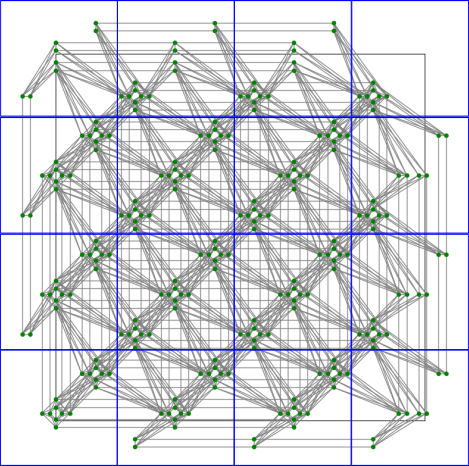
\includegraphics[width=0.7\linewidth]{p4_unitcells.png}
    \end{center}
    \caption{
        A lattice with \( 4 \times 4 \) Pegasus unit cells (\( P_4 \)).
        The D-Wave Advantage QPU is based on a lattice with \( 16 \times 16 \) Pegasus unit cells (\( P_{16} \))~\cite{dwave_topologies}.
    }
    \label{fig:p4_unitcells}
\end{figure}
\begin{figure}[!htb]
    \begin{center}
        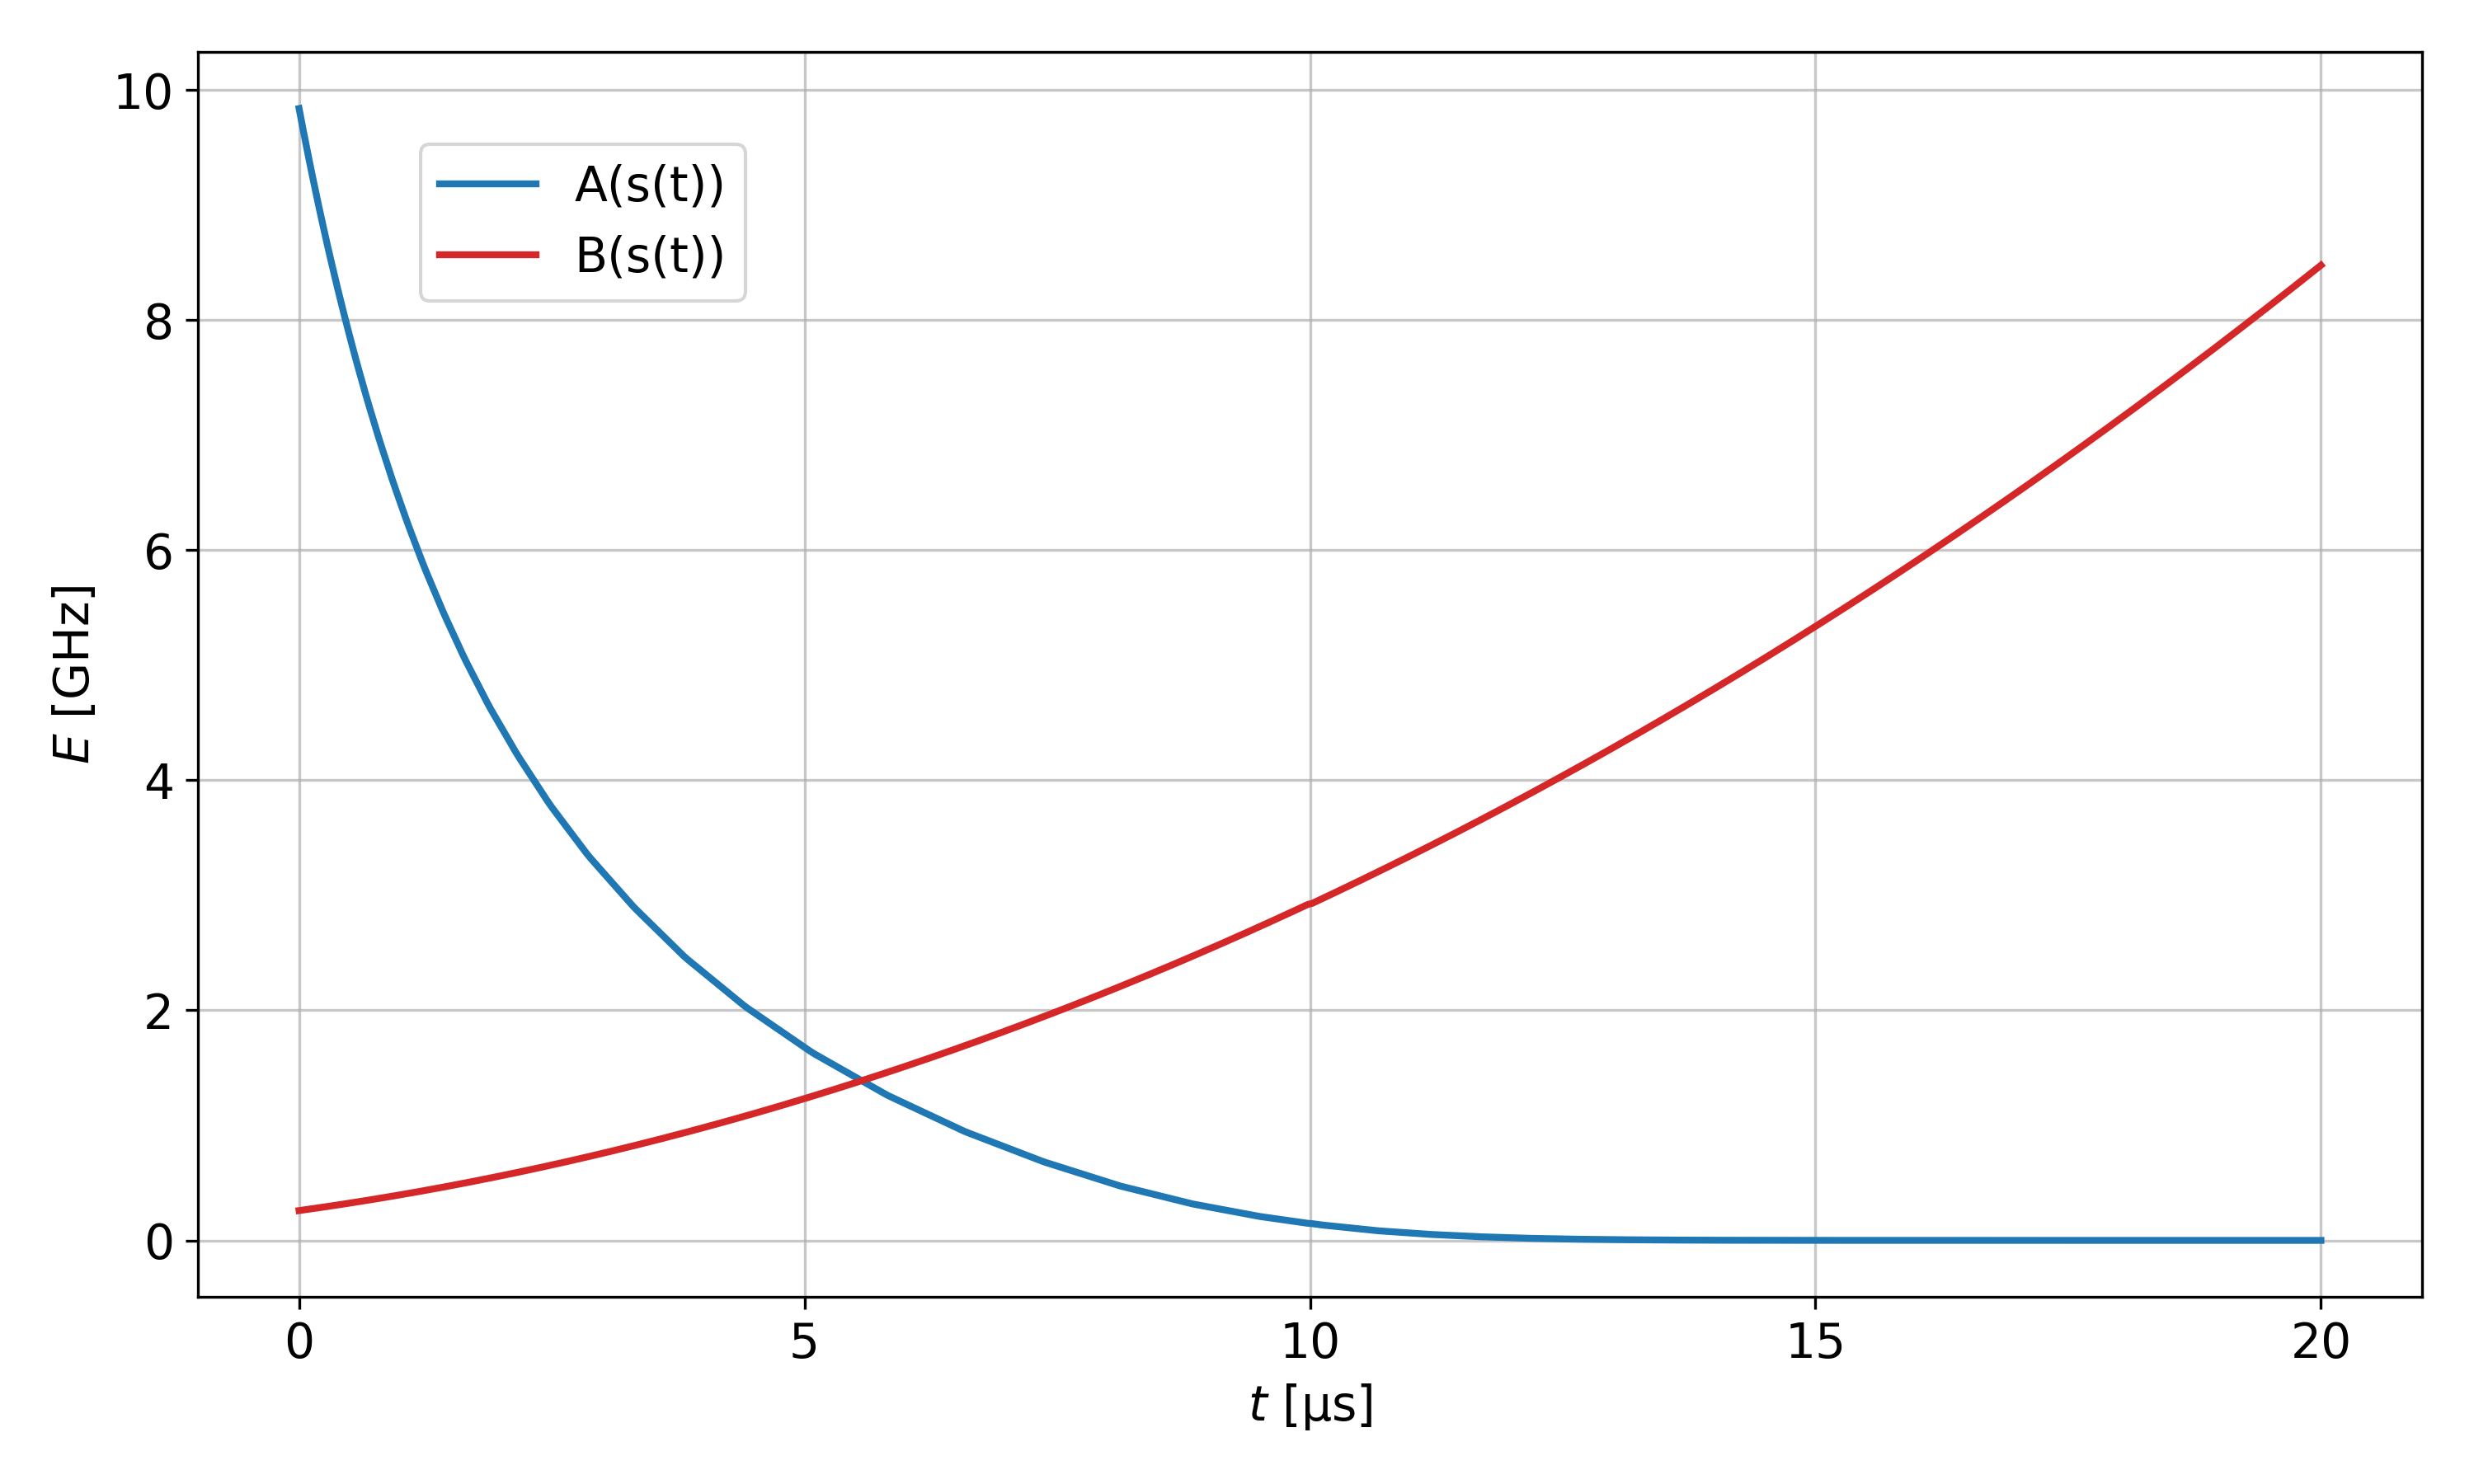
\includegraphics[width=1\linewidth]{qbm/anneal_schedules/Advantage_system4.1-s_pause=1.00-pause_duration=0.png}
    \end{center}
    \caption{
        Default anneal schedule of the D-Wave Advantage 4.1 with linear \( s(t) = t / t_a \) and \( t_a = 20 \ \si{\micro\second} \)~\cite{dwave_anneal_schedules}.
    }
    \label{fig:anneal_schedule_default}
\end{figure}

\subsubsection{Mapping the QBM to the D-Wave Quantum Annealer}
As stated in~\cite{amin_2018}, in order get a quantum annealer to sample from a quantum Boltzmann distribution, one would need to freeze the evolution at some point \( s^* \) during the annealing process and then perform the measurements.
The authors go on to say that this can be done in practice using a nonuniform \( s(t) \) that anneals slowly in the beginning, then quenches the system (completes the annealing as fast as possible) at the freeze-out point \( s^* \), if \( s^* \) is in the quasistatic regime.
In an earlier paper~\cite{amin_2015}, Amin showed that the quasistatic regime begins around 1 \si{\micro\second} for the D-Wave 2000Q, so it should not be an issue to reach the quasistatic regime for annealing times longer than 5 \si{\micro\second}.

Since a quantum annealer is a real-world physical device, samples generated with it have an associated temperature called the effective temperature.
To be more specific, the corresponding density operator is of the form
\begin{align}
    \rho(s, T) = \frac{1}{Z} e^{-\beta H(s)},
\label{eq:effective_density_operator}
\end{align}
where \( \beta = 1/kT \) is the effective inverse temperature.
In principle, \( \beta \) is an unknown quantity and must be determined in order to effectively use the annealer to generate samples from a quantum Boltzmann distribution.

Comparing the density operator of the QBM in~\cref{eq:density_operator} to the one in~\cref{eq:effective_density_operator} at the freeze-out point \( s^* \), we find
\begin{align}
\begin{split}
    \Gamma_i
        &= \beta A(s^*), \\
    b_i
        &= -\beta B(s^*) h_i, \\
    w_{ij}
        &= -\beta B(s^*) J_{ij}.
    \label{eq:qbm_scaling}
\end{split}
\end{align}
This enables us to map the QBM to the annealer if \( \beta \) can be determined to some reasonable degree of accuracy.

\subsubsection{Learning the Effective Inverse Temperature}\label{sec:learning_beta}
There is the possibility to treat \( \beta \) as a learnable parameter rather than having to choose a value empirically, as detailed by Xu and Oates in~\cite{xu_2021}.
The method is based on a log-likelihood maximization approach leading to parameter updates of the form (see \cref{app:learning_beta} for how one arrives at this result)
\begin{align}
    \Delta\betahat
        &= \frac{\eta_{\betahat}}{\betahat^2}\big(\langle E \rangle_\text{data} - \langle E \rangle_\text{model}\big),
\end{align}
where \( \betahat = 1/k\hat{T} \) is the estimator of the effective inverse temperature, and \( \eta_{\betahat} \) is the associated learning rate.
In practice, we forego the factor of \( \betahat^2 \) in the denominator for simplicity and to keep a similar form to the other gradient updates.
We must note though that this approach is only valid for classical Boltzmann distributions, but this fits our current use case as we will see in~\cref{sec:qbm_verifying_distribution}.

\subsubsection{D-Wave Ocean SDK}
D-Wave offers an easy-to-use Python package called Ocean SDK~\cite{dwave_ocean} to interact with their Leap~\cite{dwave_leap} cloud-based quantum annealing platform, which allows users to access various quantum annealers and other solvers around the globe.

One of the most important steps in solving a problem using a D-Wave annealer is finding an embedding, i.e., a mapping of the logical qubits to the physical qubits, and the SDK offers a heuristic method to do so.
If the problem cannot be directly embedded (1:1 logical:physical qubits), then a cluster of physical qubits called a chain is created to represent one logical qubit.
Chains introduce added complexity into the problem, because one then needs to tune the chain strength, i.e., the coupling constant between the qubits in the chains.
If the measured values of the qubits in a chain differ, this is called a chain break, and the system will report back the majority vote of the measured values in the chain.
Therefore, it is best to avoid chains if possible, but they are often a necessary evil for larger problems due to connectivity limitations.

Samples can be easily generated by the annealer using the \texttt{sample\_ising(h, J)} function which takes in the user-defined \( h_i \) and \( J_{ij} \) values and returns a sample set of specified size (maximum \( 10^4 \)).
The returned sample set contains the sampled state vectors (an array of shape \( (n_\text{samples}, n) \) with values \( \pm 1 \) corresponding to the qubit measurements), their energies, and other information about the run.

It must be noted that for the purposes of using a D-Wave annealer for quantum Boltzmann sampling, one must disable autoscaling to properly estimate the effective temperature, as per~\cref{eq:qbm_scaling}.
The \texttt{sample\_ising(h, J)} function has the keyword argument \texttt{autoscale=True}, which rescales the \( h_i \) and \( J_{ij} \) values by the factor~\cite{dwave_solver_parameters}
\begin{align}
\begin{split}
    r_\text{autoscale}
        = \max\Bigg\{
            &\max\bigg\{\frac{\max\{h_i\}}{\max\{h_\text{range}\}},0\bigg\},
            \max\bigg\{\frac{\min\{h_i\}}{\min\{h_\text{range}\}},0\bigg\}, \\
            &\max\bigg\{\frac{\max\{J_{ij}\}}{\max\{J_\text{range}\}},0\bigg\},
            \max\bigg\{\frac{\min\{J_{ij}\}}{\min\{J_\text{range}\}},0\bigg\}
        \Bigg\}.
\end{split}
\end{align}
This is because the main use case of D-Wave annealers is to maximize the probability of measuring the ground state, thus the problem is rescaled so that the \( h_i \) and \( J_{ij} \) values fully utilize the allowed range of values, essentially decreasing the effective temperature; therefore we set \texttt{autoscale=False} to avoid this.
For the Advantage 4.1 system the allowed value ranges are \( h_\text{range} = [-4, 4] \) and \( J_\text{range} = [-1, 1] \)~\cite{dwave_solver_properties}.

\subsubsection{Generating More Robust Statistics}\label{sec:gauge}
QPUs are not perfect, and sometimes specific qubits or parts of the chip might have readout biases.
One can perform a gauge transformation on the problem to mitigate such issues.
If we have an \( n \)-qubit problem, then we can generate a random vector \( \vec{r} \in \{+1, -1\}^n \) which allows us to change the submission to the solver without actually changing the underlying problem.
This is done by taking
\begin{align}
\begin{split}
    h_i
        &\rightarrow r_i h_i, \\
    J_{ij}
        &\rightarrow r_i r_j J_{ij}, \\
    (s_1, \dots, s_n)
        &\rightarrow (r_1 s_1, \dots, r_n s_n),
\end{split}
\end{align}
and then transforming the results back using the third relation above, where \( s_i \) is the measured value of qubit \( i \).

\subsubsection{Previous Work in This Field}
In recent years, a number of researchers have dabbled in using D-Wave quantum annealers to train Boltzmann machines~\cite{adachi_2015,benedetti_2016,anschuetz_2019,wiebe_2019,rocutto_2020,dixit_2021,ilmo_2021,wilson_2021,xu_2021}.
The most common approach is to train a classical RBM with quantum assistance, i.e., using the annealer to generate the samples in the negative phase rather than using Gibbs sampling.
Classical RBMs trained with quantum assistance are a special case of the QBM, i.e., when \( s^* = 1 \) the problem reduces to a classical RBM, as \( \lim_{s\rightarrow 1} \Gamma_i = 0 \) in~\cref{eq:qbm_scaling}.

One thing that stands out the most about some of the previous research is that very few discuss embeddings and anneal schedules, which as we will see in the next section are important for getting the best possible performance out of the annealer.
Therefore, we aim to create a basic framework with which one can use to approach the problem of using a D-Wave annealer to sample from a (quantum) Boltzmann distribution.

\section{12-Qubit Problem}\label{sec:qbm_12_qubit_problem}
In order to get a better understanding of how the QBM works, we study a small 12-qubit problem that can be solved exactly.
For this purpose we take a QBM with restrictions in both the visible and hidden layers and train it using the log-likelihood lower bound maximization approach; we call this a bound-based quantum restricted Boltzmann machine, or BQRBM for short.
We configure the model with 8 visible and 4 hidden units to act as a regularized autoencoder.

\subsection{Sampling From a Quantum Boltzmann Distribution}
Before training the model, we first need to assess the Advantage 4.1's ability to sample from quantum Boltzmann distributions.
To this end, we randomly generate the values of \( h_i \) and \( J_{ij} \) from a normal distribution with \( \mu = 0 \) and \( \sigma = 0.1 \), then use the KL divergence to compare samples generated by the Advantage 4.1 with theoretical distributions.

\subsubsection{Anneal Schedule Format}
The \( A(s) \) and \( B(s) \) values for a D-Wave annealer are fixed and depend on the specific system~\cite{dwave_anneal_schedules}, but the Ocean SDK allows us to define a nonuniform \( s(t) \) using a list of \( (t, s) \) tuples, which then determine the \( A(s(t)) \) and \( B(s(t)) \) curves.
In this section we use what we call pause-and-quench anneal schedules that
\begin{enumerate}
    \item start at \( (t = 0, s = 0) \),
    \item paus the system at \( (\tpause, \spause) \) for a duration of \( \Deltapause \),
    \item quench the system at \( (\tquench, \squench) \) over a duration of \( \Deltaquench \).
\end{enumerate}
Thus, the anneal schedules provided to the solver are of the form
\begin{align}
    [
        (0, 0),
        (\tpause, \spause),
        (\tquench, \squench),
        (\tquench + \Deltaquench, 1)
    ],
\end{align}
where
\begin{align}
\begin{split}
    \squench &\equiv \spause, \\
    \tpause &= \spause \cdot \trelative, \\
    \tquench &= \tpause + \Deltapause.
\end{split}
\end{align}
An annotated example of a custom pause-and-quench anneal schedule with \( \squench = 0.55 \), \( \trelative = 20 \ \si{\micro\second} \), and \( \Deltapause = 10 \ \si{\micro\second} \) is given in~\cref{fig:anneal_schedule_annotated}.
\begin{figure}[!htb]
    \begin{center}
        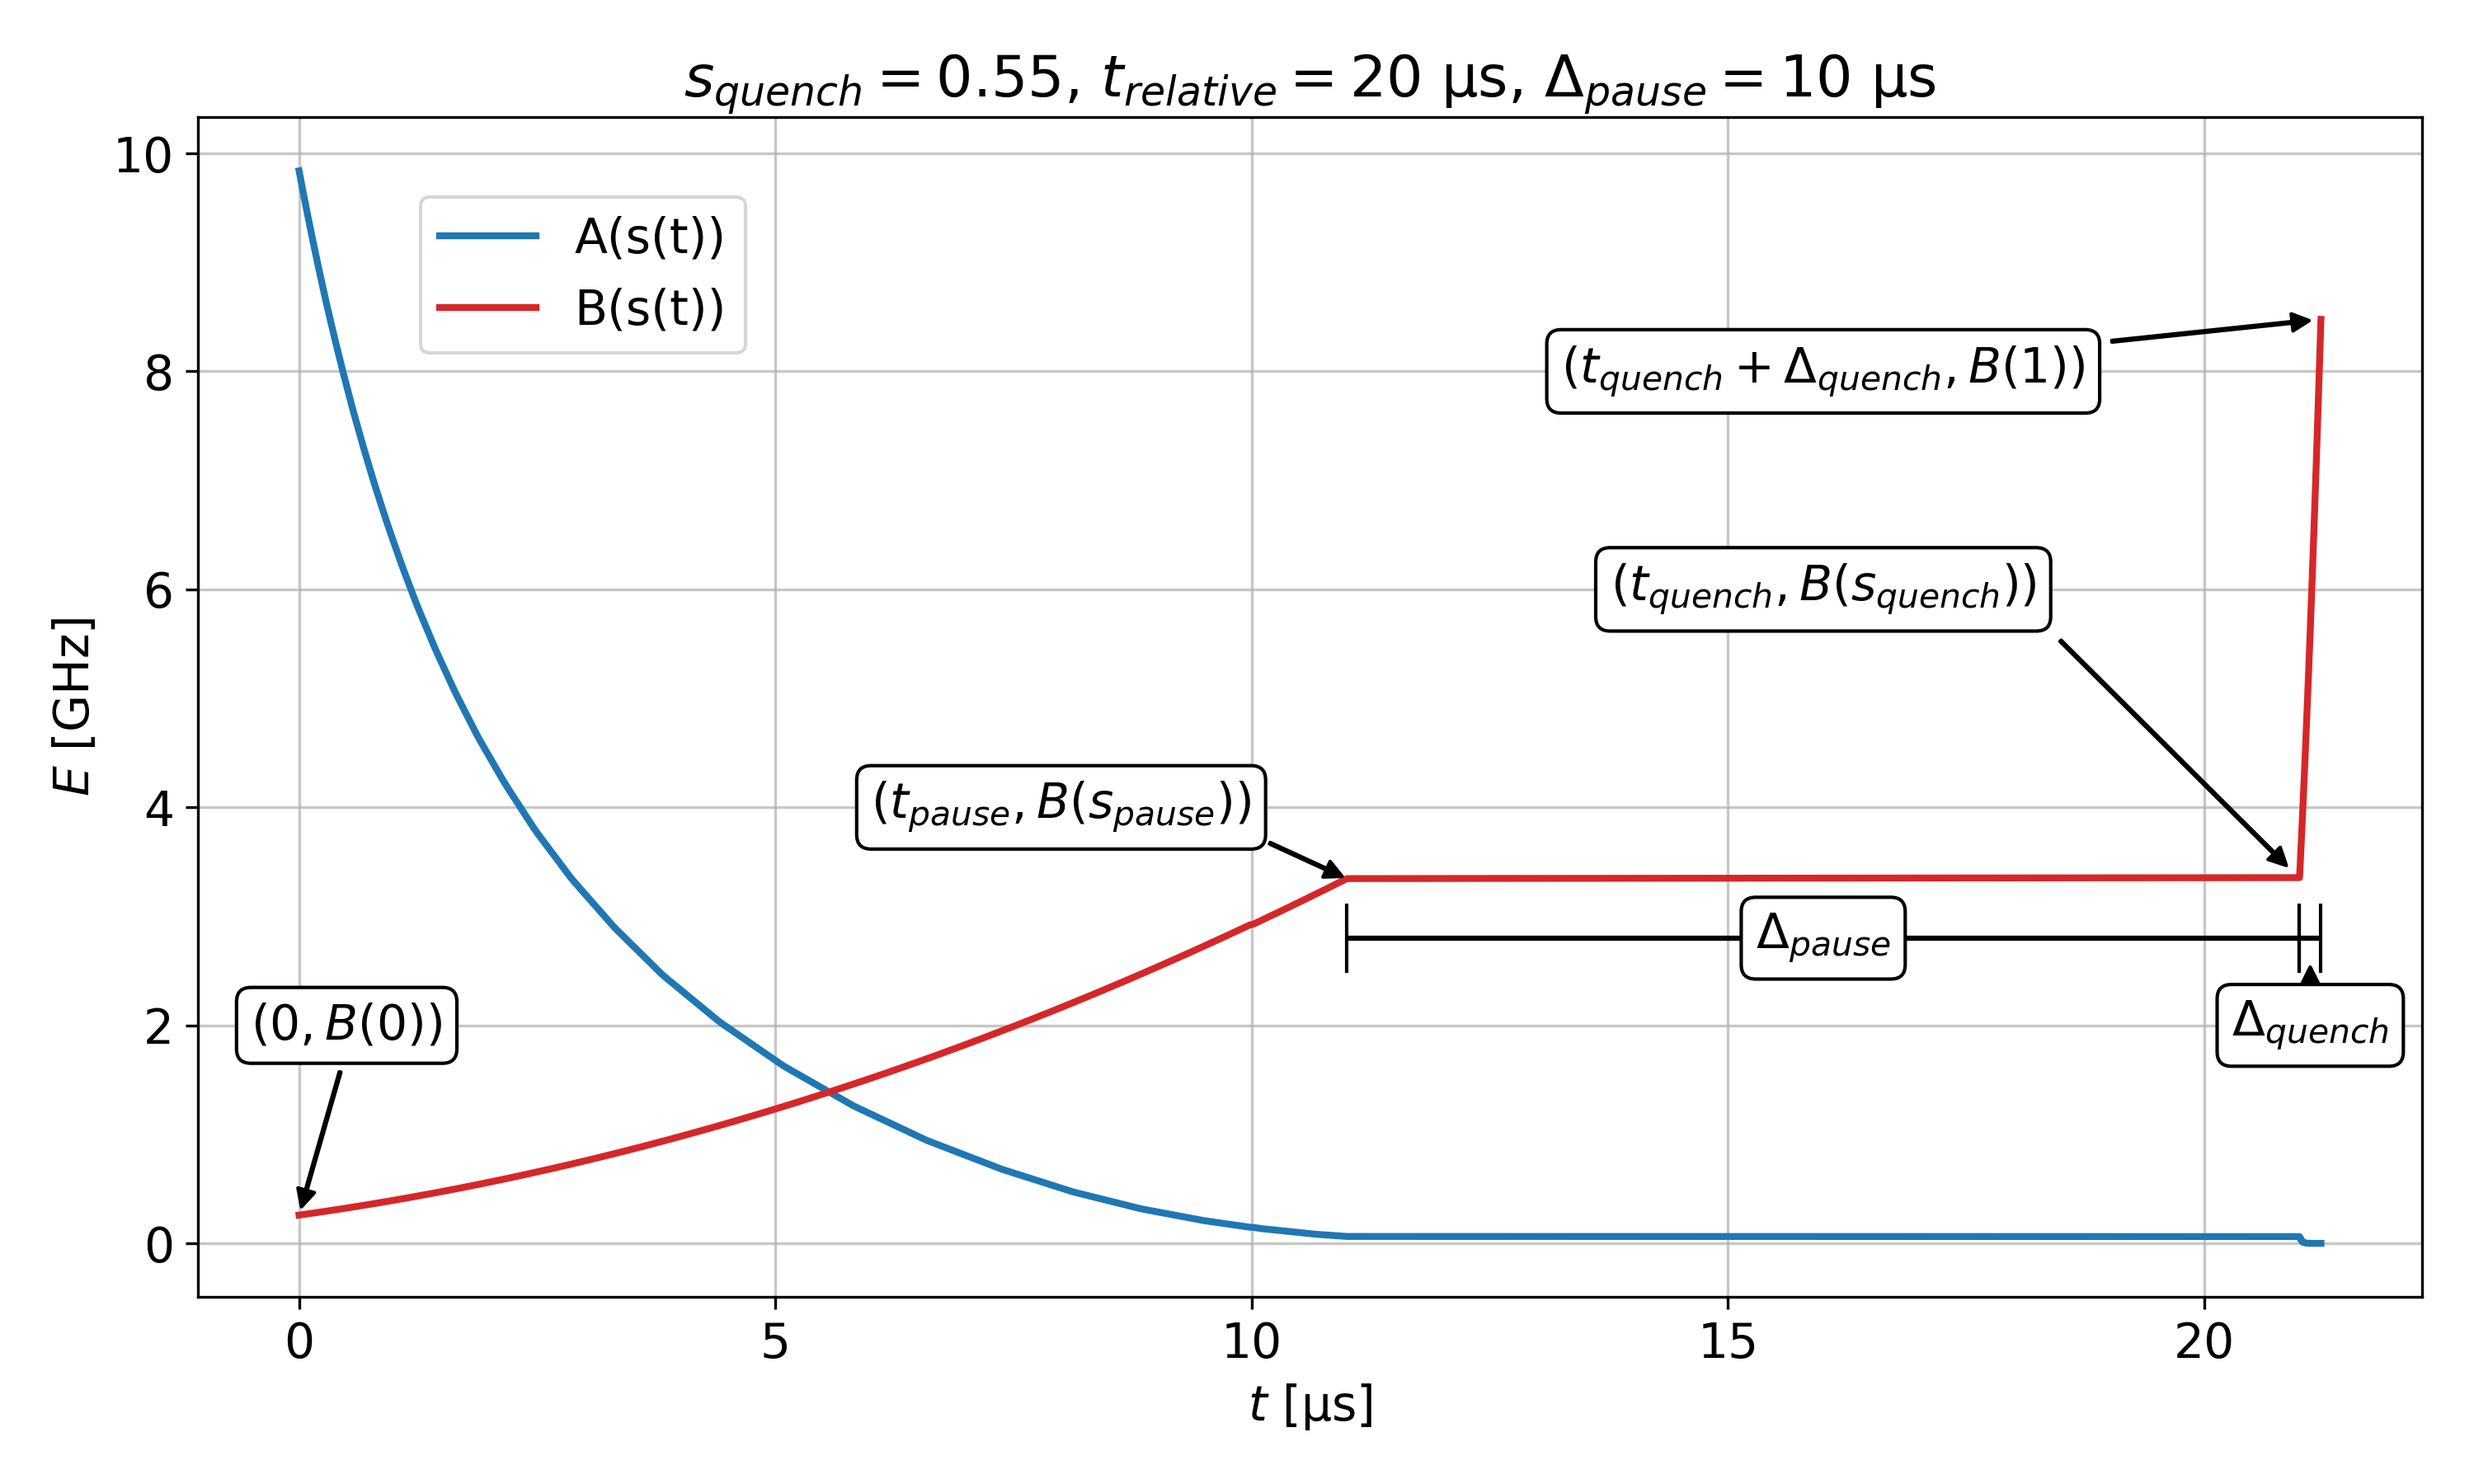
\includegraphics[width=1\linewidth]{qbm/anneal_schedules/Advantage_system4.1-s_pause=0.55-pause_duration=10.png}
    \end{center}
    \caption{
        Example of a custom pause-and-quench anneal schedule for the D-Wave Advantage 4.1~\cite{dwave_anneal_schedules}.
        Annotations indicate the points \( (t, B(s(t))) \), as well as the periods over which the annealing is paused and quenched.
    }
    \label{fig:anneal_schedule_annotated}
\end{figure}

The minimum quench duration \( \Deltaquench \) is a function of \( \squench \) and is limited by the system's fastest anneal rate \( \alphaquench \)
\begin{align}
    \Deltaquench(\squench) = \frac{1 - \squench}{\alphaquench}.
\end{align}
The Advantage 4.1 system allows a maximum of \( \alphaquench = 2 \ \si{\micro\second}^{-1} \)~\cite{dwave_solver_parameters}.

\subsubsection{Verifying the Distribution}\label{sec:qbm_verifying_distribution}
We use the KL divergence \( \DKL{\ptheory}{\psamples} \) to compare the probabilities of the energies computed from the samples returned by the Advantage 4.1 with the theoretical energy distributions for \( s = 0.01, 0.02, \dots, 1 \) and \( T = 10^{-3}, 2, 4, \dots, 200 \ \si{\milli\kelvin} \), which we visualize as heatmaps in~\cref{fig:dkl_min_heatmap}.
More information on how the KL divergences are computed can be found in~\cref{app:kl_divergence_in_practice}, how the density matrix (from which the theoretical distributions are obtained) is computed in~\cref{app:exact_rho_computation}, and the required constants in~\cref{app:constants}.

In the right heatmap, where \( \squench = 0.55 \), we observe a narrow band in which the Advantage 4.1-generated samples closely resemble a quantum Boltzmann distribution, and in fact the samples approximate multiple distributions depending on the effective temperature.
Marshall et al. present similar results using a D-Wave 2000Q in~\cite{marshall_2019}, in which they discuss if the distribution returned by the annealer fits that of a quantum Boltzmann distribution late in the anneal process when \( A(s^*) / B(s^*) \ll 1 \), then the distribution at \( s^* \) should be close to a classical Boltzmann distribution, i.e.,
\begin{align}
    e^{-\beta H(s^*)} \approx e^{-\beta B(s^*) H_\text{final}}.
\end{align}
This in turn means that not only is there one optimal \( s^* \) and effective temperature which models the distribution, but rather a set of them corresponding to a family of distributions for which \( \beta B(s^*) \) is constant.
Therefore, this explains the streak pattern in the heatmaps.

Furthermore, we observe that the left heatmap, where \( \squench = 0.25 \), is quite similar to the right one where \( \squench = 0.55 \), but with higher KL divergence values and temperatures.
This indicates that quenching at \( \squench = 0.25 \) produces samples that are distributed more as a classical Boltzmann distribution, and that we cannot generate samples from quantum Boltzmann distributions with \( s^* \lessapprox 0.45 \), at least with the anneal schedules we use here.

\begin{figure}[!htb]
    \begin{center}
        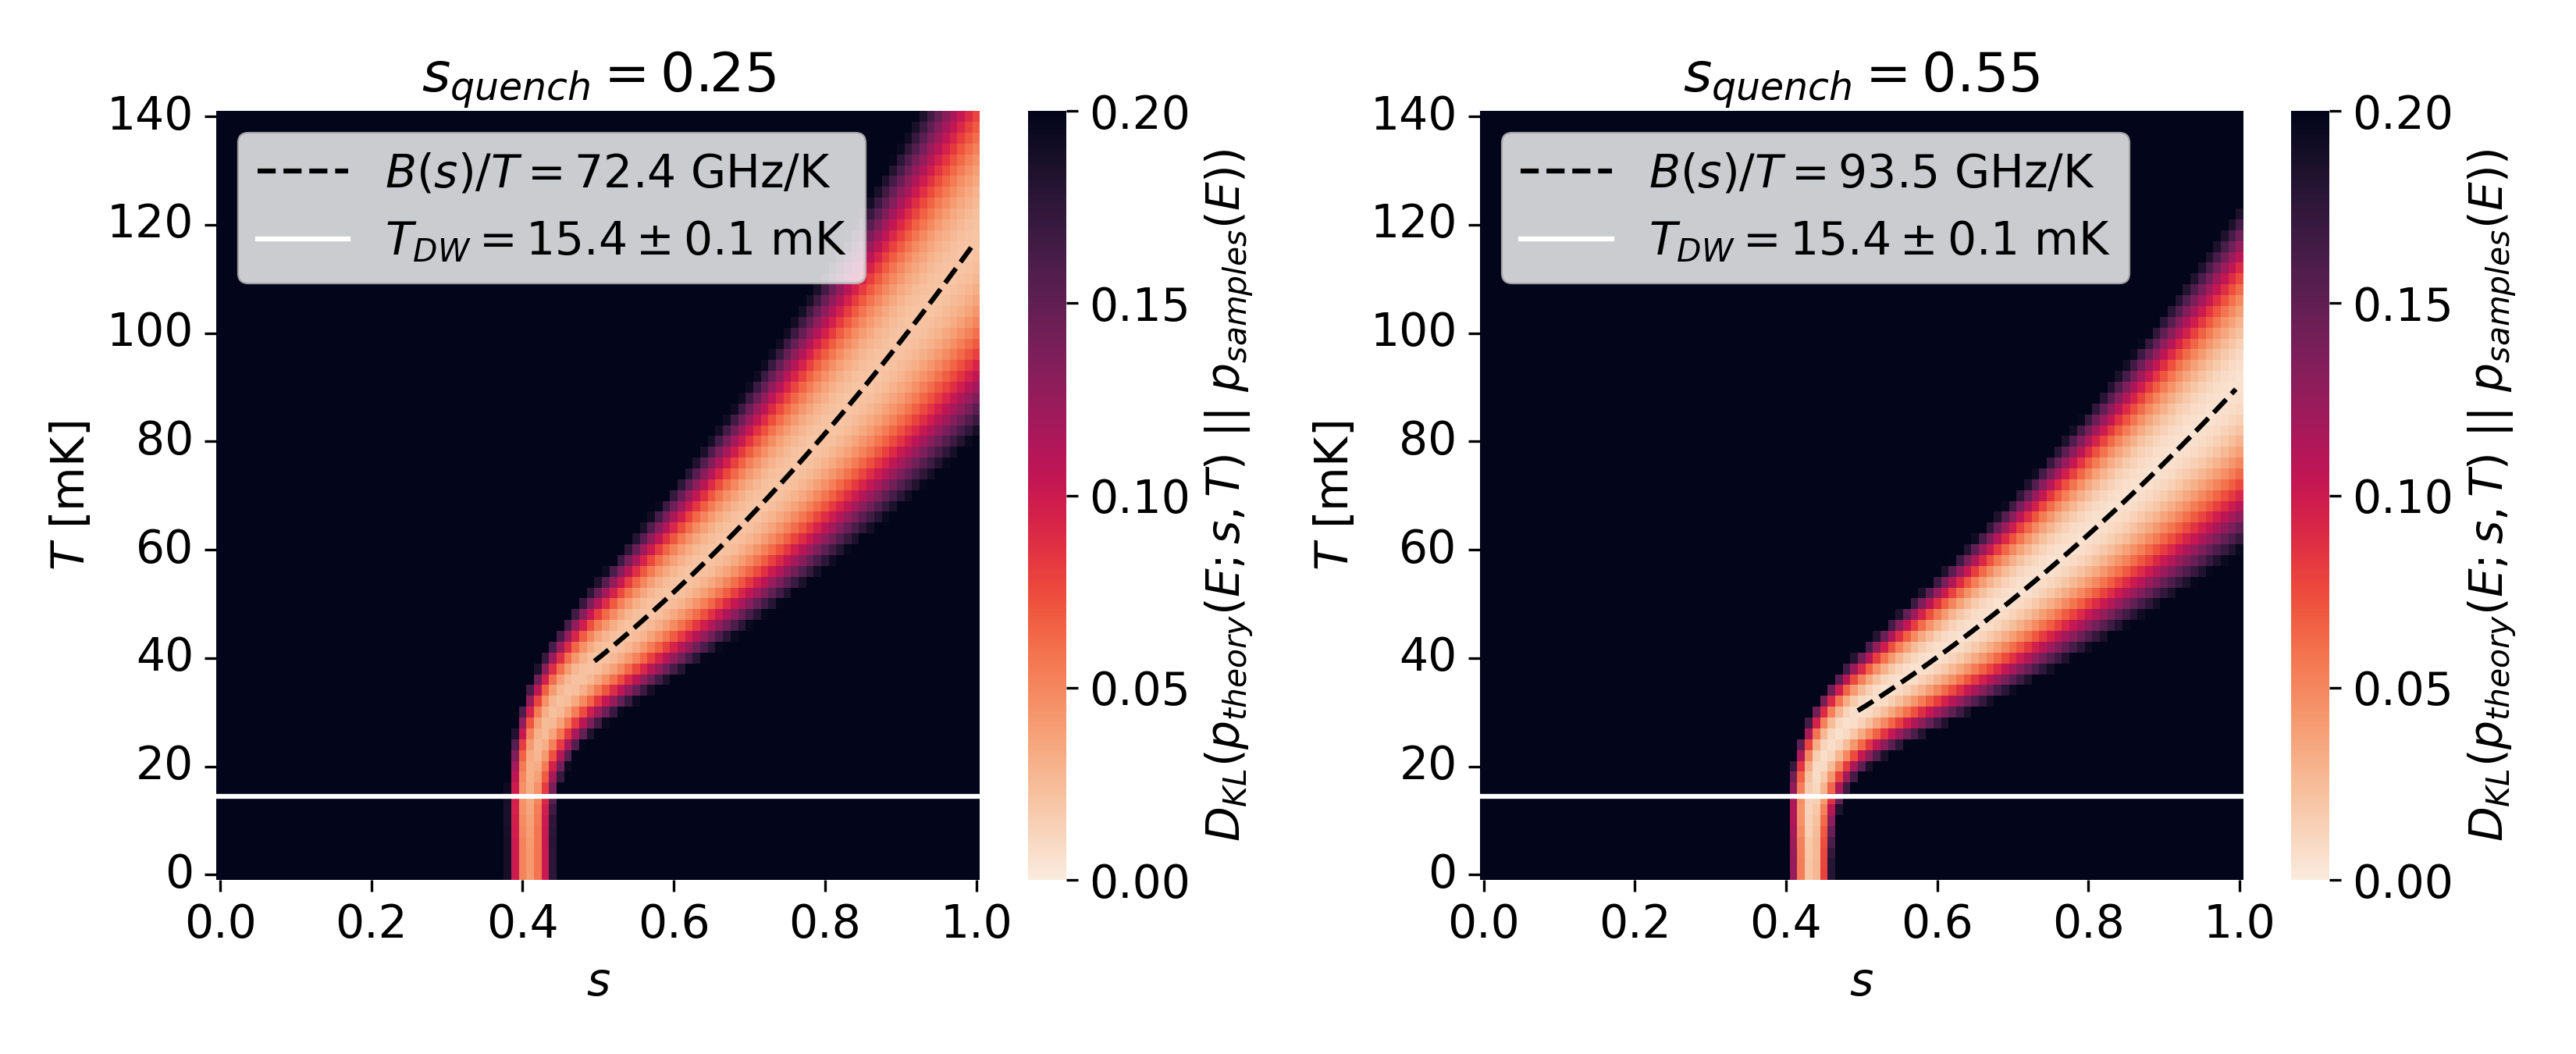
\includegraphics[width=1\linewidth]{qbm/8x4/embedding_comparison/config_05/dkl_min_heatmap-embedding=10.png}
    \end{center}
    \caption{
        Heatmaps of \( \DKL{\ptheory}{\psamples} \) comparing the distribution produced by samples from the D-Wave Advantage 4.1 to a set of theoretical QBM distributions for two different quench points using embedding 10.
        The dashed lines represent the optimal values of \( B(s) / T = \text{constant} \), computed by taking the value of \( T \) which produces the lowest KL divergence for each \( s \ge 0.5 \).
        Data represents an ensemble average over 10 random gauge sample sets consisting of \( 10^4 \) samples each.
    }
    \label{fig:dkl_min_heatmap}
\end{figure}

It must also be noted that the effective temperature corresponding to the classical Boltzmann distribution \( (s^* = 1) \) is significantly higher than that of the D-Wave temperature of \( T_\text{DW} = 15.4 \pm 0.1 \ \si{\milli\kelvin} \)~\cite{dwave_leap}\footnote{Temperature obtained from the system properties in the Leap interface.}.
It is not entirely clear exactly why the effective temperature of the distribution is so much higher than the device temperature, but in~\cite{marshall_2019} they give several possible reasons, including the discrepancy between the temperature of the device and the qubits, fluctuations in the temperature while annealing, and control errors masquerading as higher temperatures.
In principle, higher effective temperatures are unwanted because they shrink the range of allowed values for the weights and biases as per~\cref{eq:qbm_scaling}, but there is not much one can do about this.

From analysis of the heatmaps and the fact that we cannot produce distributions with \( s^* \lessapprox 0.45 \), we conclude that nontrivial dynamics occur while the system is quenching, i.e., the system cannot quench fast enough.
It is difficult to compare directly since the 2000Q is a different system than the Advantage 4.1 we study here, but in~\cite{marshall_2019} they also allude to the possibility of nontrivial dynamics occurring.
The 2000Q allows for quenching with \( \alphaquench = 1 \), which is only a factor of two smaller than that of the Advantage 4.1.
Therefore, if as supposed in~\cite{marshall_2019} that the quench is not fast enough, then likely such a small difference in how fast the system can be quenched would not drastically change the results.

If we take a second to think about it, the qubits are oscillating at a frequency in terms of gigahertz.
This means that a quench duration of a few hundred nanoseconds still allows for a number of oscillations in the qubits, which is likely enough time for nontrivial dynamics to take place.
It would be interesting to verify via simulation how fast a quench must be in order to freeze out the distribution at the desired point \( s^* \).

We conclude that we are unable to reliably generate arbitrary quantum Boltzmann distributed samples using the Advantage 4.1 system.
Therefore, for the remainder of this thesis we focus on training models with \( s^* = 1 \) using classical Boltzmann distributed samples generated by the Advantage 4.1, also enabling us to use the aforementioned method of learning the effective temperature.

\subsubsection{Choosing an Embedding}
We compare 10 different heuristically generated embeddings based on how well they approximate the desired distribution.
In this embedding comparison, we use only direct embeddings (no chains), so the embeddings only differ by the location of the qubits on the chip, and pause-and-quench anneal schedules with \( \trelative = 20 \ \si{\micro\second} \) and \( \Deltapause = 0 \ \si{\micro\second} \).

It is difficult to compare the heatmaps of all embeddings and quench points due to the higher dimensionality of the data, so we take the minimum KL divergence over \( s \) and \( T \), and plot it as a function of \( \squench \) in~\cref{fig:dkl_mins_embeddings}.
We immediately see how varied the results are depending on the embedding and quench point, highlighting the importance of choosing a good embedding and anneal schedule.

\begin{figure}[!htb]
    \begin{center}
        \includegraphics[width=1\linewidth]{qbm/8x4/embedding_comparison/config_05/kl_divergence_mins.png}
    \end{center}
    \caption{
        Comparison of \( \min_{s,T}\big\{\DKL{\ptheory}{\psamples}\big\} \) for different embeddings and \( \squench \) values.
        Data represents an ensemble average over 10 random gauge sample sets consisting of \( 10^4 \) samples each.
        Shaded regions represent one standard deviation.
    }
    \label{fig:dkl_mins_embeddings}
\end{figure}

Our findings indicate that embedding 10 is likely a good choice because it produces the best results at \( \squench = 0.55 \).
The rest of the results in this subsection use embedding 10.

\subsubsection{Choosing an Anneal Schedule}\label{sec:choosing_an_anneal_schedule}
With the chosen embedding we want to see if there is a way in which we can alter the anneal schedule to further reduce the KL divergence.
We start with the same anneal schedule formula as before, except we introduce pausing before initiating the quench for durations \( \Deltapause = 0, 10, 100 \ \si{\micro\second} \), as well as the addition of \( \trelative = 100 \ \si{\micro\second} \).

\begin{figure}[!htb]
    \begin{center}
        \includegraphics[width=1\linewidth]{qbm/8x4/exact_analysis/config_05/embedding_10/kl_divergence_mins.png}
    \end{center}
    \caption{
        Comparison of \( \min_{s,T}\big\{\DKL{\ptheory}{\psamples}\big\} \) for various pause-and-quench anneal schedules using embedding 10.
        Data represents an ensemble average over 10 random gauge sample sets consisting of \( 10^4 \) samples each.
        Shaded regions represent one standard deviation.
        Some of the sample sets with longer annealing times and pause durations had less than \( 10^4 \) samples as to satisfy the maximum allowed run time of the D-Wave Advantage 4.1.
    }
    \label{fig:dkl_mins_embedding_05}
\end{figure}

\cref{fig:dkl_mins_embedding_05} illustrates that pausing and longer annealing times has little effect, and that quenching in the range of \( \squench \in [0.55, 0.6] \) produces the best results.
With this information, we opt to use an anneal schedule with \( \squench = 0.55 \), \( \trelative = 20 \ \si{\micro\second} \), and \( \Deltapause = 0 \ \si{\micro\second} \), as it offers a good balance between performance and QPU usage time.

\subsection{Training Data}
Having verified that the Advantage 4.1 can indeed produce Boltzmann distributed samples to some degree of accuracy, we proceed with training models using both a simulation and the Advantage 4.1.
We randomly generate a training data set consisting of 1500 samples, 1000 from a \( \mathcal{N}(-2, 1) \) distribution and 500 from a \( \mathcal{N}(3, 1) \) distribution, visualized in~\cref{fig:hist_data}.
\begin{figure}[!htb]
    \begin{center}
        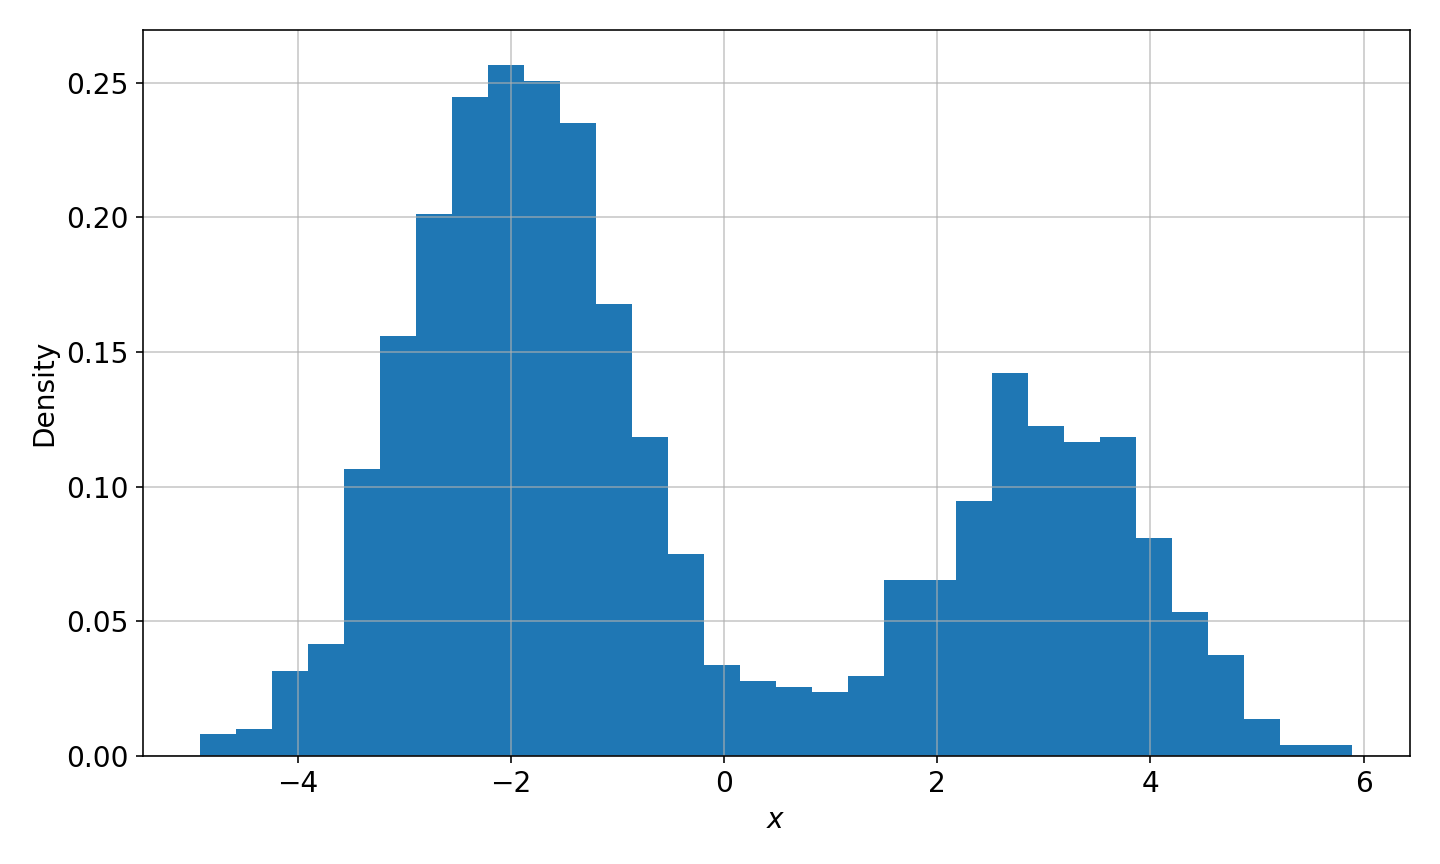
\includegraphics[width=1\linewidth]{qbm/8x4/Advantage_system4.1/hist_data.png}
    \end{center}
    \caption{
        Histogram of the training data set used in the 12-qubit problem.
    }
    \label{fig:hist_data}
\end{figure}

\subsection{Simulation-based Model}
The first step is training a model using a simulation in which the samples are generated using the probabilities obtained from computing \( \rho \) exactly.
Here we use a mini-batch size of 10, \( s^* = 1 \), and an initial learning rate of \( \eta = 0.1 \) with a schedule that exponentially decays the learning rate every 10 epochs by a factor of 2 beginning at epoch 50 as defined in~\cref{app:lr_exp_decay}.
The learning rate \( \eta_{\hat{\beta}} \) for the parameter \( \betahat \) follows a similar schedule, except it has a decay period of 20 as opposed to 10, to allow for more range of motion in the \( \betahat \) parameter later in the training process if the estimate needs to adapt more quickly to a new effective \( \beta \).

\subsubsection{Results}\label{sec:qbm_simulation_results}
\cref{fig:train_results_exact} shows the results of training the simulation-based model on the aforementioned data set.
We use the KL divergence \( \DKL{\pdata}{\pmodel} \) as a way to track the progress of the training and get a read on how well the model learns the data set distribution, because minimizing the KL divergence is equivalent to maximizing the log-likelihood~\cite{murphy_2012}.
The KL divergence is computed at the end of every epoch using a sample set of size \( 10^4 \).
In the left plot of \cref{fig:train_results_exact}, we observe a clear trend of the KL divergence being minimized.
The learning curve reaches an optimal value after about 80 epochs, then remains steady for the next 20 epochs until the end of training.

\begin{figure}[!htb]
    \begin{center}
        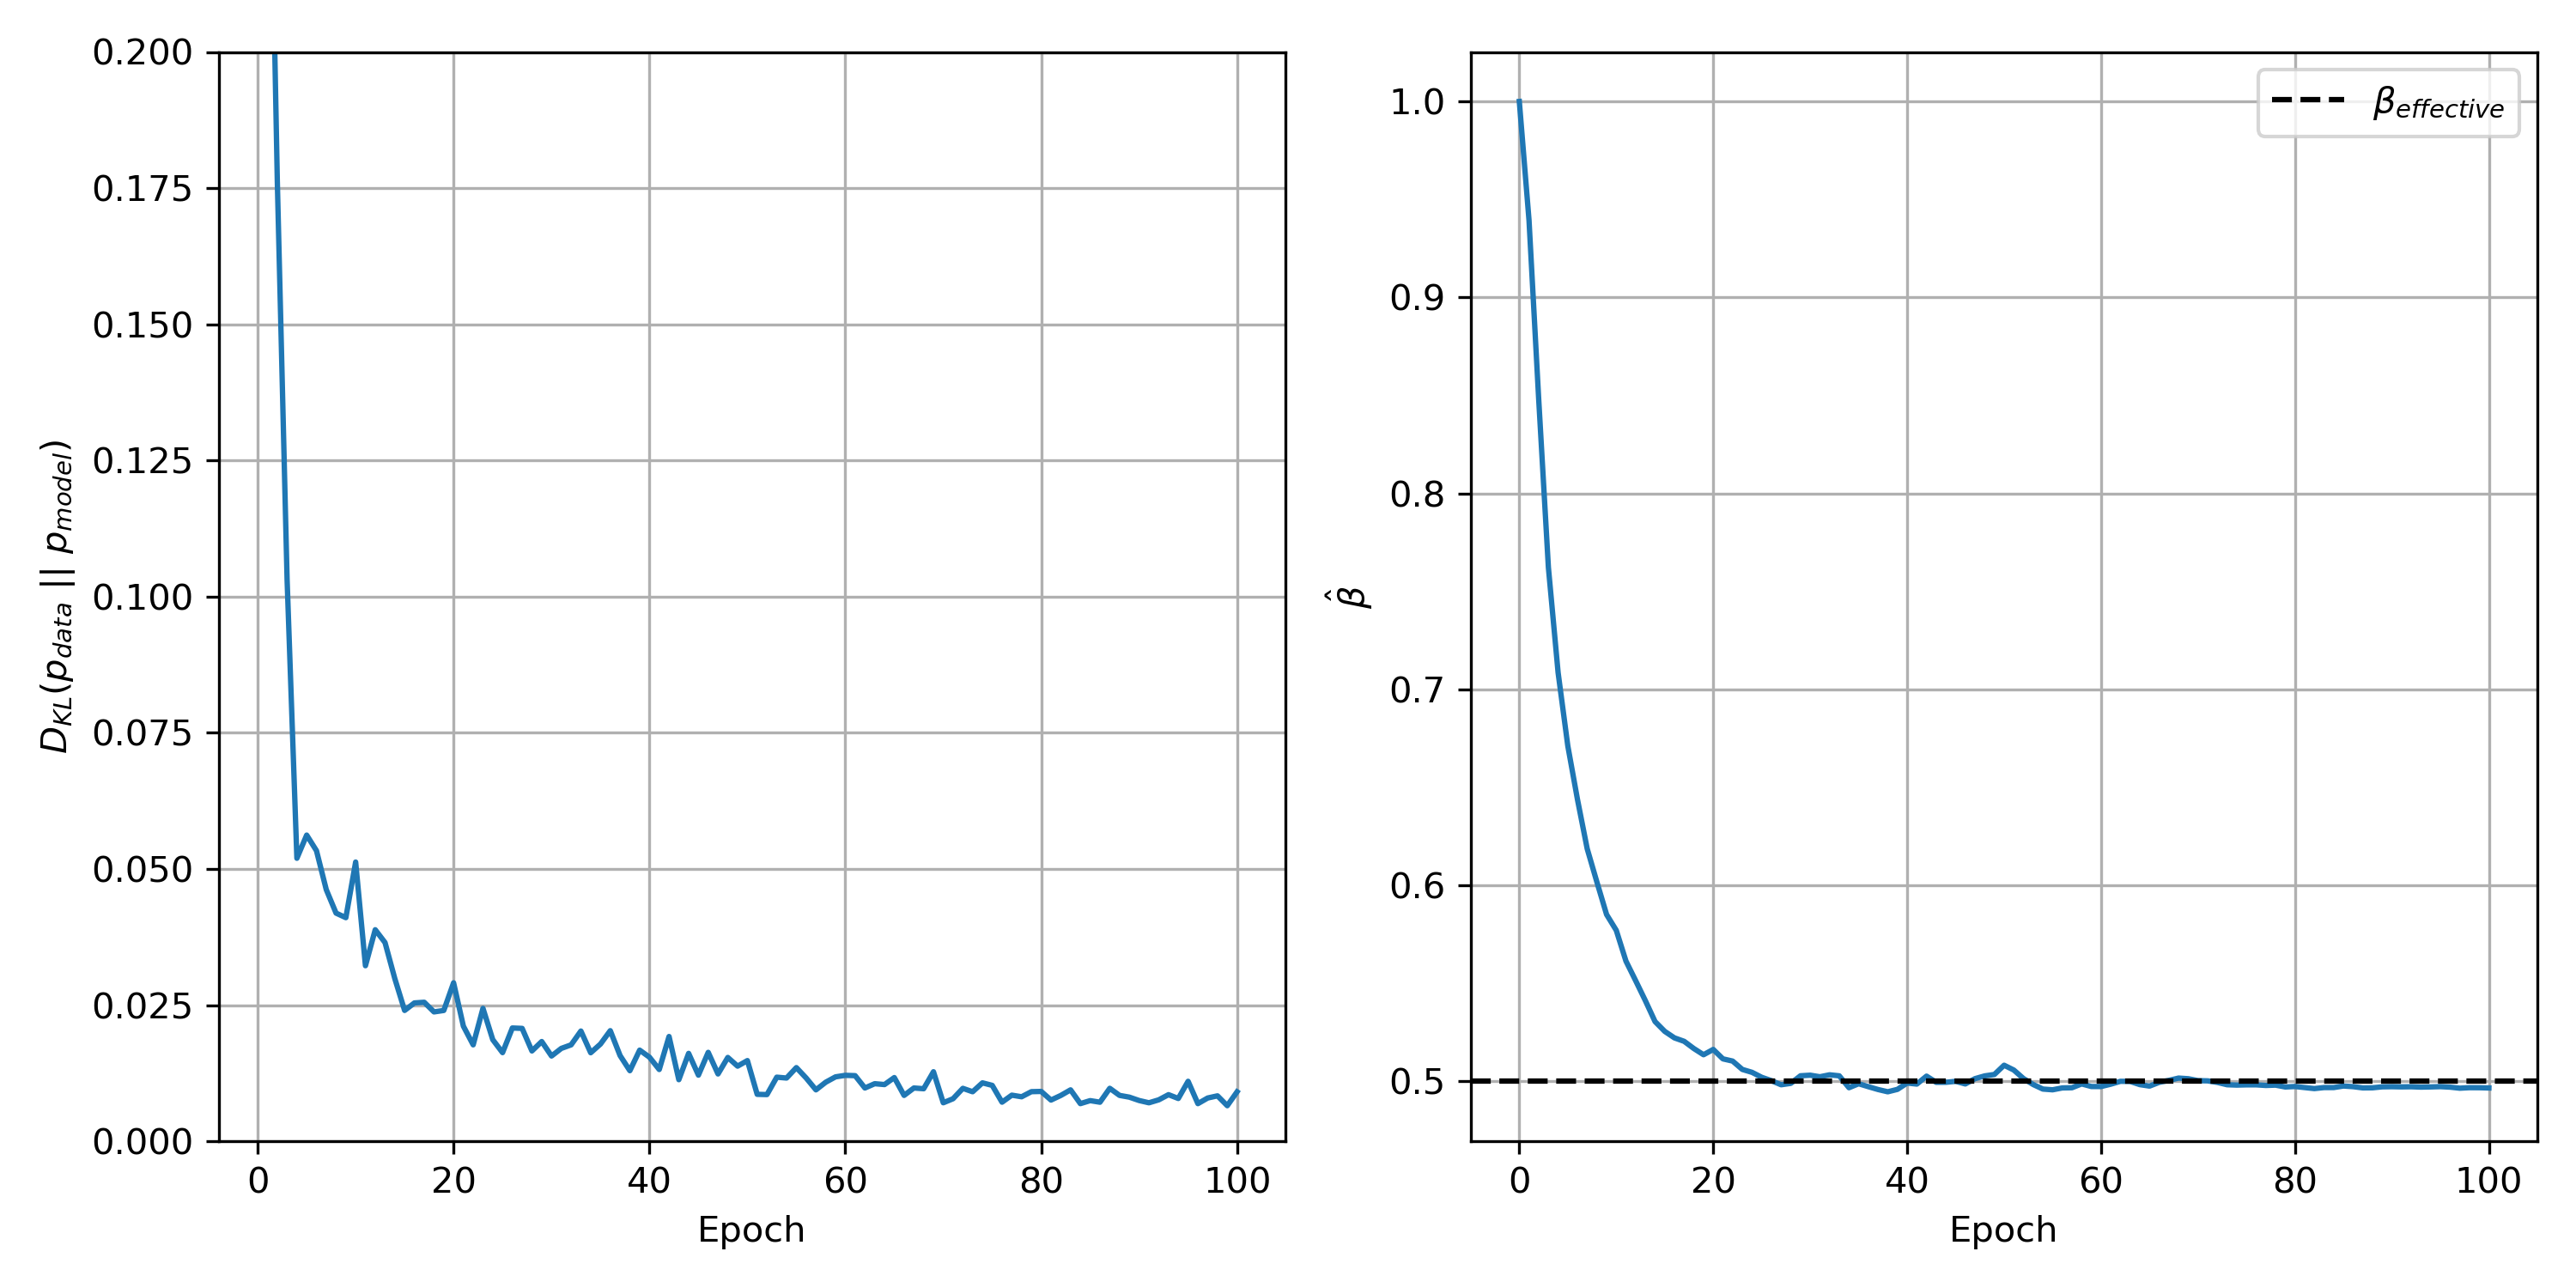
\includegraphics[width=1\linewidth]{qbm/8x4/Advantage_system4.1/train_results_exact.png}
    \end{center}
    \caption{
        Training results of the 12-qubit model trained using the simulation.
        On the left is the KL divergence \( \DKL{\pdata}{\pmodel} \) plotted against the epochs; each data point was generated using \( 10^4 \) samples at the end of every epoch.
        On the right is the learned temperature estimator \( \hat{T} \) plotted against the epochs, as well as the effective temperature that the simulation was configured to generate samples at.
    }
    \label{fig:train_results_exact}
\end{figure}

We designed the simulation such that we can set the effective \( \beta \) to any value we desire.
To verify that the model can learn an accurate value for the estimator \( \betahat \), we configure the simulation to generate samples at an effective value of \( \beta = 0.5 \ \si{\giga\hertz}^{-1} \ (T \approx 96 \ \si{\milli\kelvin}) \) and initialize the model with a value of \( \betahat = 1 \ \si{\giga\hertz}^{-1} \ (\hat{T} \approx 48 \ \si{\milli\kelvin}) \).
The results in the right plot of~\cref{fig:train_results_exact} confirm that it is able to learn a value of \( \betahat \) close to the actual effective \( \beta \).

Overall, the results show that the model can generate samples similar to the training distribution reasonably well when trained using the simulation, i.e., the best case scenario.
Additionally, we are able to verify that the model can accurately learn an estimate of the effective temperature.
We use the results of this model as a baseline to compare the models trained using the Advantage 4.1 in the next subsection with.

\subsection{D-Wave Advantage 4.1-based Model}
Having successfully trained the 12-qubit BQRBM using samples generated via exact simulation, we move to switching the sample generation part to the Advantage 4.1.
We take the same hyperparameters as the simulation, and an anneal schedule using \( \squench = 0.55 \), \( \trelative = 20 \ \si{\micro\second} \), and \( \Deltapause = 0 \ \si{\micro\second} \).
We see in~\cref{fig:dkl_min_heatmap} that \( \squench = 0.55 \) has an optimal temperature of around 90 \si{\milli\kelvin} for \( s^* = 1 \), thus we take \( \betahat = 0.5 \ \si{\giga\hertz}^{-1} \ (\hat{T} \approx 96 \ \si{\milli\kelvin}) \) as our initial guess for the effective \( \beta \), and let the model learn from there.

\subsubsection{Results}\label{sec:qbm_annealer_results}
The KL divergences in~\cref{fig:train_results_annealer} and~\cref{tbl:12_qubit_qbm_KL_divergences} show the model trained using the Advantage 4.1 produces samples that resemble the training distribution to some extent, but still underperforms when compared with the simulation and the classically trained RBM.
This is possibly due to the information loss associated with using the D-Wave to approximate the distribution, which likely arises due to noise and errors (see~\cref{sec:challenges}), because after all, real-world systems governed by quantum mechanics are highly sensitive to their environment.
\begin{figure}[!htb]
    \begin{center}
        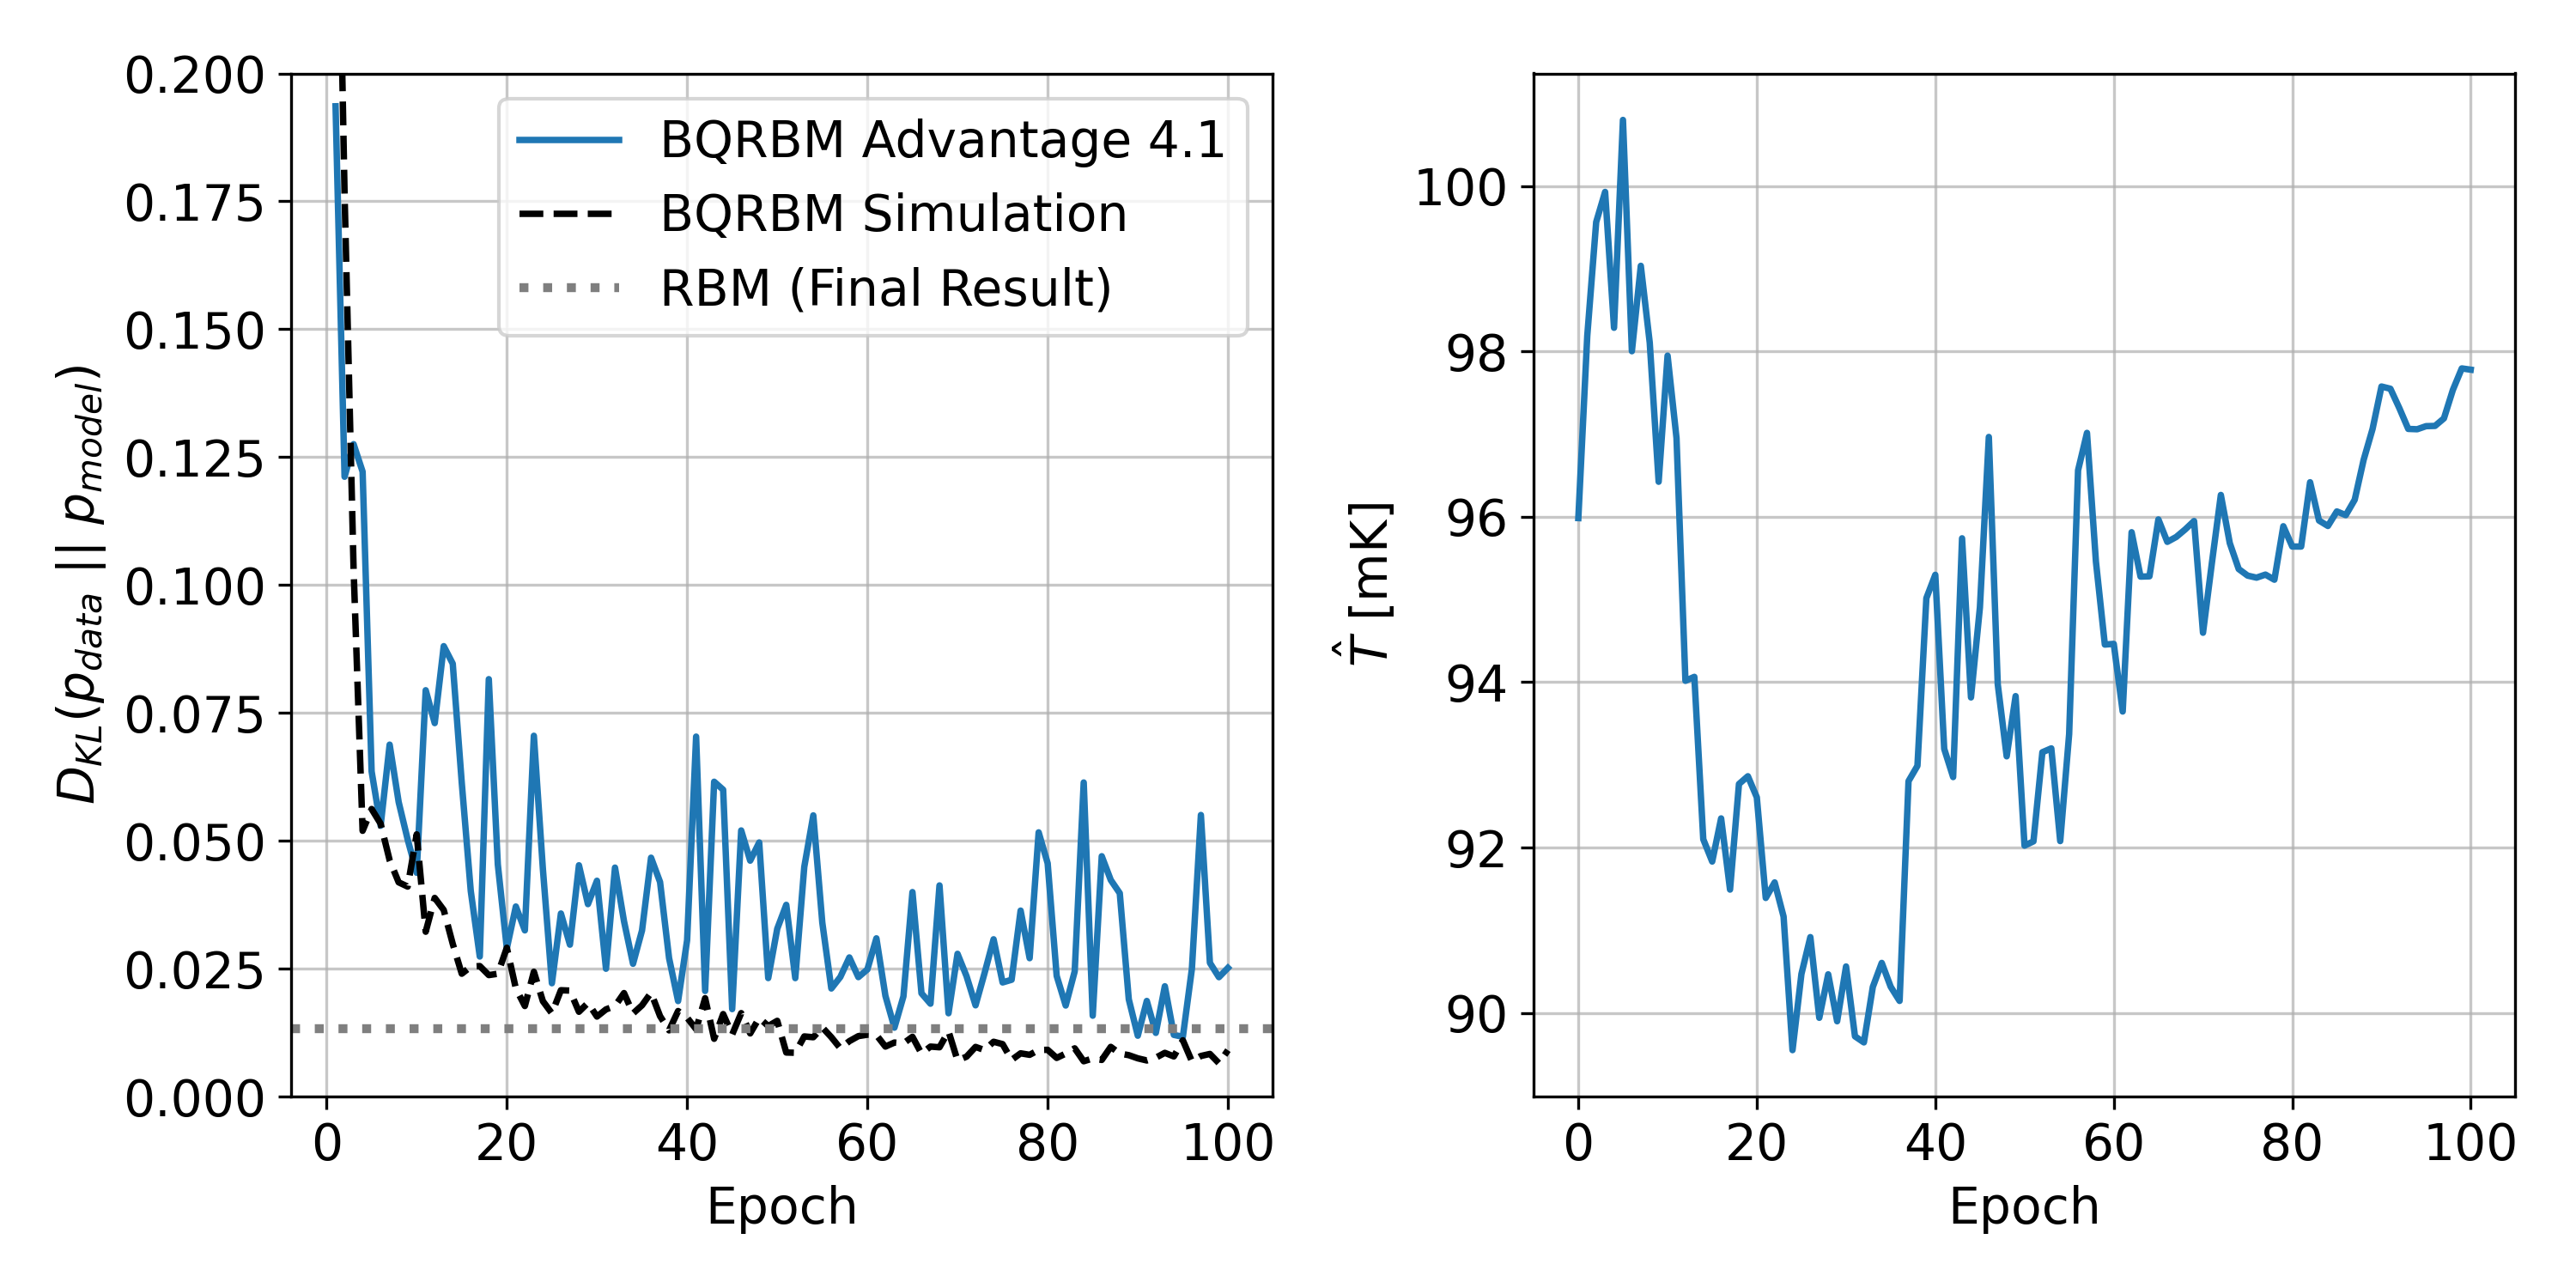
\includegraphics[width=1\linewidth]{qbm/8x4/Advantage_system4.1/train_results_annealer.png}
    \end{center}
    \caption{
        Training results of the 12-qubit model trained using samples generated with the D-Wave Advantage 4.1 compared with that of the simulation and the final results of a classical RBM.
        On the left is the KL divergence \( \DKL{\pdata}{\pmodel} \) plotted against the epochs; each data point was generated using \( 10^4 \) samples at the end of every epoch.
        On the right is the learned temperature estimator \( \hat{T} \) plotted against the epochs.
    }
    \label{fig:train_results_annealer}
\end{figure}

\begin{table}[!htb]
    \centering
    \begin{adjustbox}{max width=\textwidth}
        \input{../tables/qbm/12_qubit_kl_divergences.tbl}
    \end{adjustbox}
    \caption{
        KL divergences of the 12-qubit BQRBM models vs.~the classical RBM.
        The values are shown in the format mean \(\pm\) one standard deviation from an ensemble of 100 sample sets consisting of \( 10^4 \) samples each.
}
    \label{tbl:12_qubit_qbm_KL_divergences}
\end{table}

We notice that the Advantage 4.1-based model struggles most with the trough between the two Gaussian peaks in the training distribution based on the Q-Q plots in~\cref{fig:qq_comparison}.
\begin{figure}[!htb]
    \begin{center}
        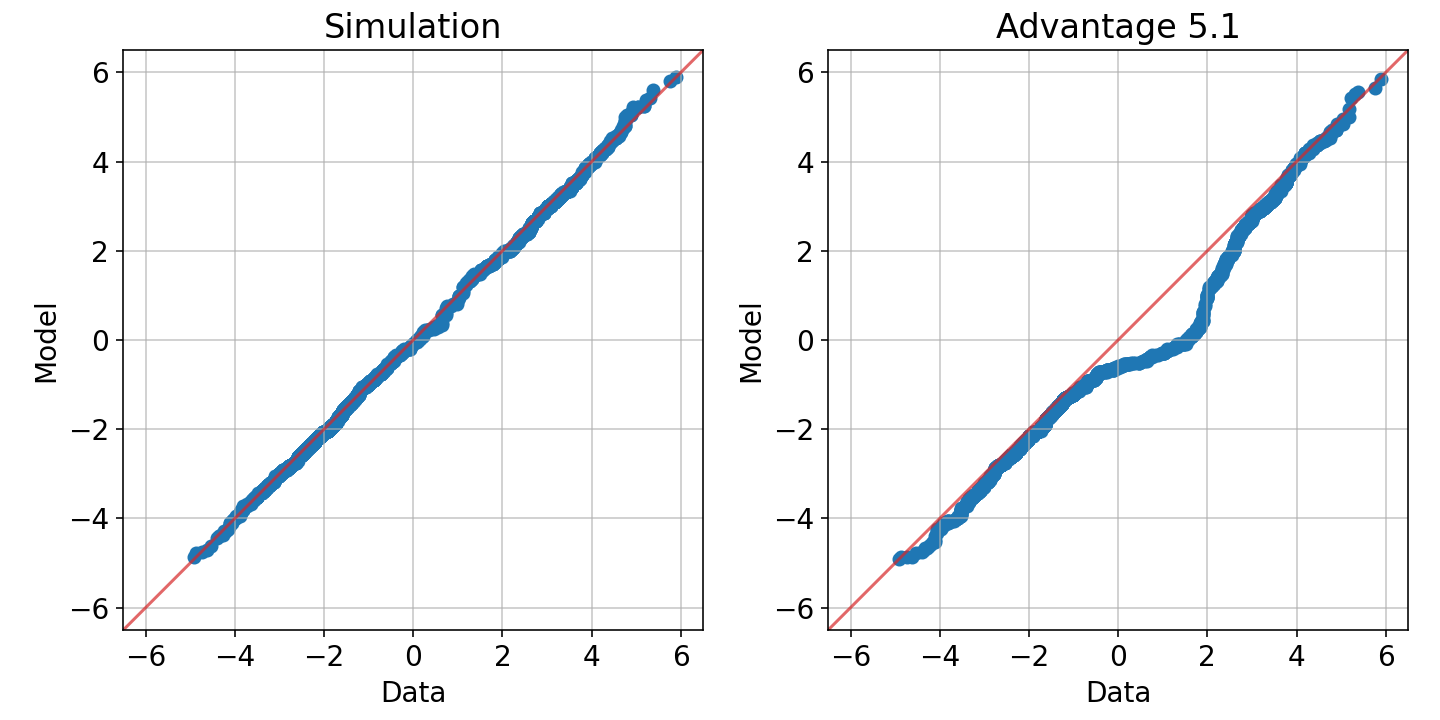
\includegraphics[width=1\linewidth]{qbm/8x4/Advantage_system4.1/qq_comparison.png}
    \end{center}
    \caption{Log return Q-Q plots of the 12-qubit model trained using the simulation (left) and the D-Wave Advantage 4.1 (right).}
    \label{fig:qq_comparison}
\end{figure}

Although we cannot track the true effective temperature throughout the training process, we are able to see how close the learned effective temperature estimate at the end matches that generated by samples using the final learned weights and biases.
The heatmap shown in \cref{fig:learned_effective_temperature} confirms that the Advantage 4.1-based model's \( \betahat \) value of \( 97.8 \ \si{\milli\kelvin} \) is quite close to the \( 95.6 \ \si{\milli\kelvin} \) computed from the optimal \( B(s) / T \) value.
\begin{figure}[!htb]
    \begin{center}
        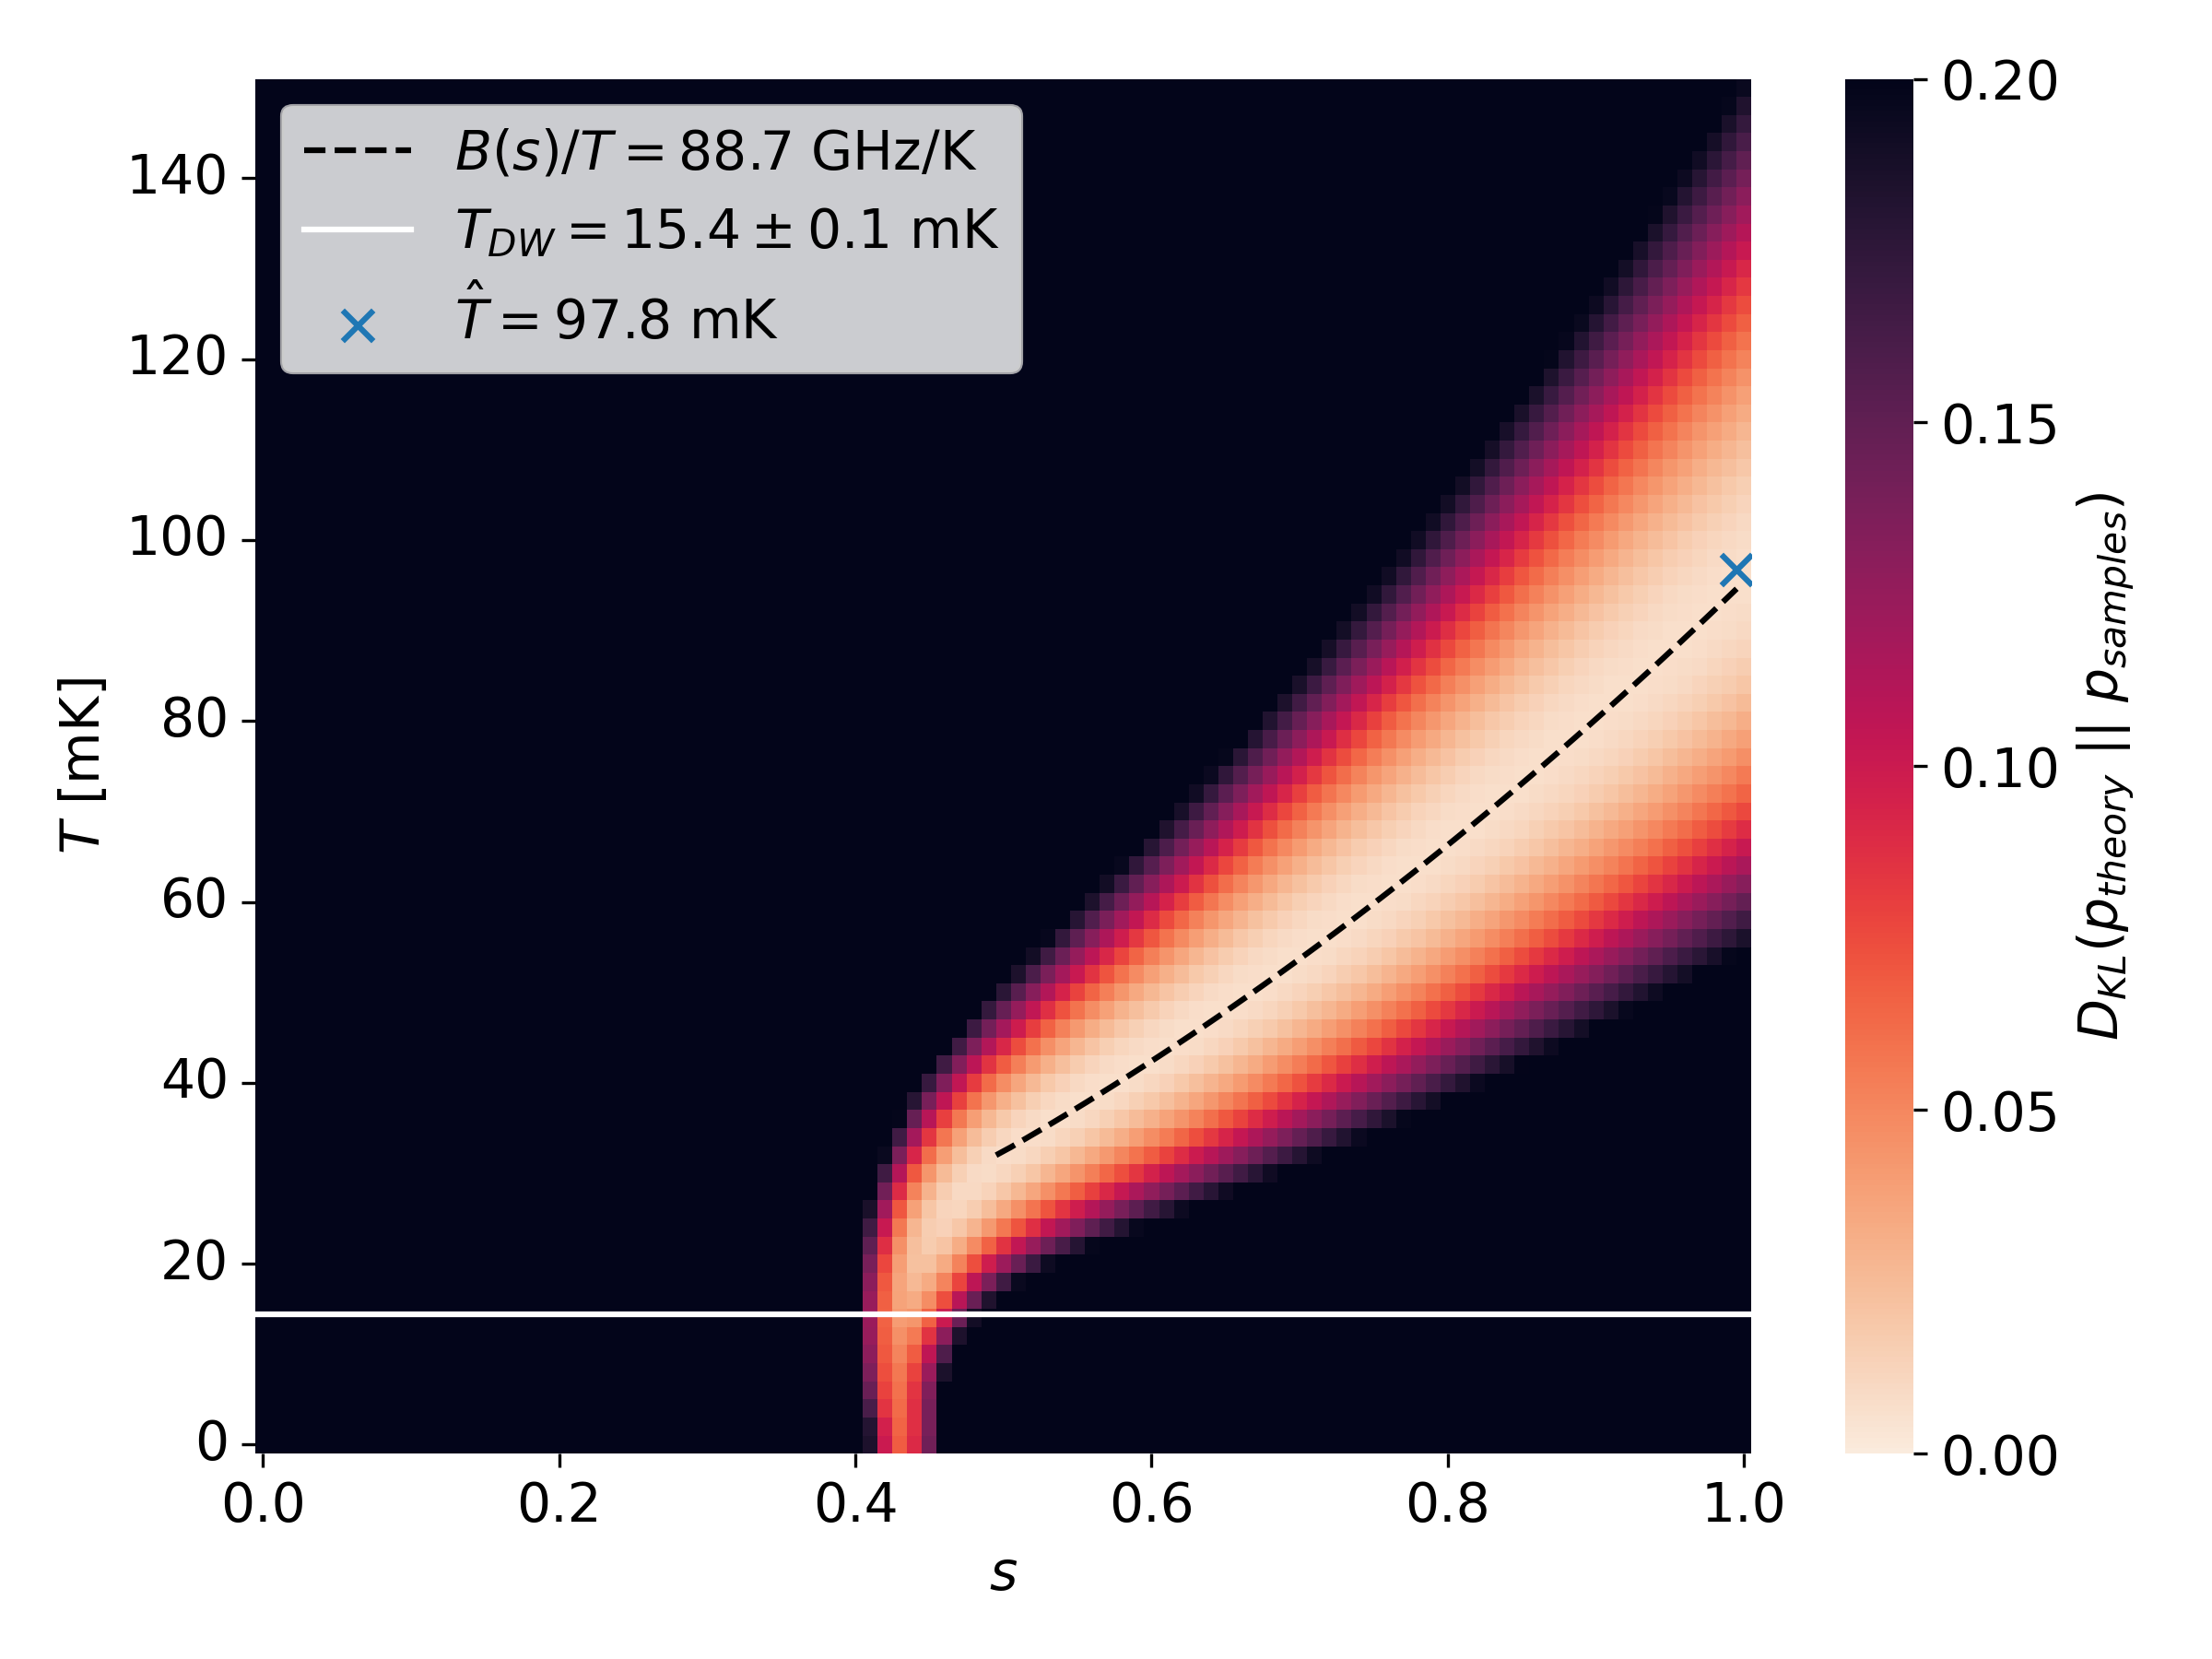
\includegraphics[width=0.7\linewidth]{qbm/8x4/Advantage_system4.1/effective_temperature.png}
    \end{center}
    \caption{
        Heatmap of \( \DKL{\ptheory}{\psamples} \) comparing the distributions produced by samples from the Advantage 4.1 to a set of theoretical QBM distributions, using the final \( h_i \) and \( J_{ij} \) values learned by the 12-qubit model trained using the Advantage 4.1.
        The blue cross indicates the learned estimate of the effective temperature.
        The dashed line represents the optimal value of \( B(s) / T = \text{constant} \), computed by taking the value of \( T \) which produces the lowest KL divergence for each \( s \ge 0.5 \).
        Data represents an ensemble average over 10 random gauge sample sets consisting of \( 10^4 \) samples each.
    }
    \label{fig:learned_effective_temperature}
\end{figure}

The results in this section show that a BQRBM can indeed be trained using a D-Wave quantum annealer.
The 12-qubit problem played a crucial role in our understanding of how one can use a D-Wave quantum annealer to generate Boltzmann distributed samples.
Although the results are not spectacular, and underperform the simulation and classical model, they still show promise.
It will be interesting to rerun this analysis on the next generation of D-Wave quantum annealers to see how much they improve.

\section{The Quantum Market Generator}\label{sec:quantum_market_generator}
With deeper insights into the workings of the BQRBM from the 12-qubit problem, we move to the final stage of training a quantum market generator with 64 visible and 30 hidden units.
All results in this section use the same baseline data set (B) as in~\cref{sec:classical_market_generator}.

\subsection{Setting the Annealer's Hyperparameters}\label{sec:qbm_hyperparameters}
Unlike the 12-qubit problem, the larger problem restricts our ability to perform an in-depth analysis to compare the sample distributions produced by the Advantage 4.1 with that of theory.
Therefore, we have to take a more practical approach when choosing some of the annealer hyperparameters such as the relative chain strength, quench point, and embedding.
To this end, we train a number of models with various settings of these hyperparameters for 20 epochs to get a read on the trend direction, and then choose their values empirically.
For this, we use a mini-batch size of 10, \( s^* = 1 \), constant learning rates of \( \eta = 0.02 \) and \( \eta_{\hat{\beta}} = 0.01 \), and an initial value of \( \betahat = 0.25 \ \si{\giga\hertz}^{-1} \ (\hat{T} \approx 192 \ \si{\milli\kelvin}) \).

The reason we only train for 20 epochs is that the epoch duration is quite high (10-25 minutes) due to latency and load on the annealer, ergo it is not very feasible to train every model for a higher number of epochs.
With an average epoch duration of around 15 minutes, a model trained for 20 epochs takes roughly 5 hours, so training for 100 epochs would take around a day.

\subsubsection{Choosing a Relative Chain Strength}\label{sec:qbm_rcs}
The chain strength \( \gamma \) is computed using the relative chain strength \( \rcs \) as
\begin{align}
    \gamma
        &= \rcs \cdot \min\Big\{
            \max\{J_\text{range}\}, \max\big\{\{\abs{h_i}\} \cup \{\abs{J_{ij}}\}\big\}
        \Big\}.
\end{align}

We train models using various values of \( \rcs \in [0.3, 2] \), and a pause-and-quench anneal schedule with \( \squench = 0.55 \), \( \trelative = 20 \ \si{\micro\second} \), and \( \Deltapause = 0 \ \si{\micro\second} \).
The results are plotted in~\cref{fig:qbm_log_returns_rcs_comparison} (only a subset depicted).
We find that too low values of \( \rcs \) lead to more chain breaks early on in the training process, which then cause the model to learn a higher temperature, in turn shrinking the allowed range of weights and biases to the point where the model can no longer learn effectively.
Everything indicates that higher relative chain strengths produce better results.
After a number of epochs, we observe \( \max\big\{ \{\abs{h_i}\} \cup \{\abs{J_{ij}}\} \big\} \) grow to a value larger than 0.5, implying that values of \( \rcs \ge 2 \) would not change the results since \( \gamma \) is reaching its limit of \( \max\{J_\text{range}\} = 1 \).
Therefore, we choose a value of \( \rcs = 2 \).

\begin{figure}[!htb]
    \begin{center}
        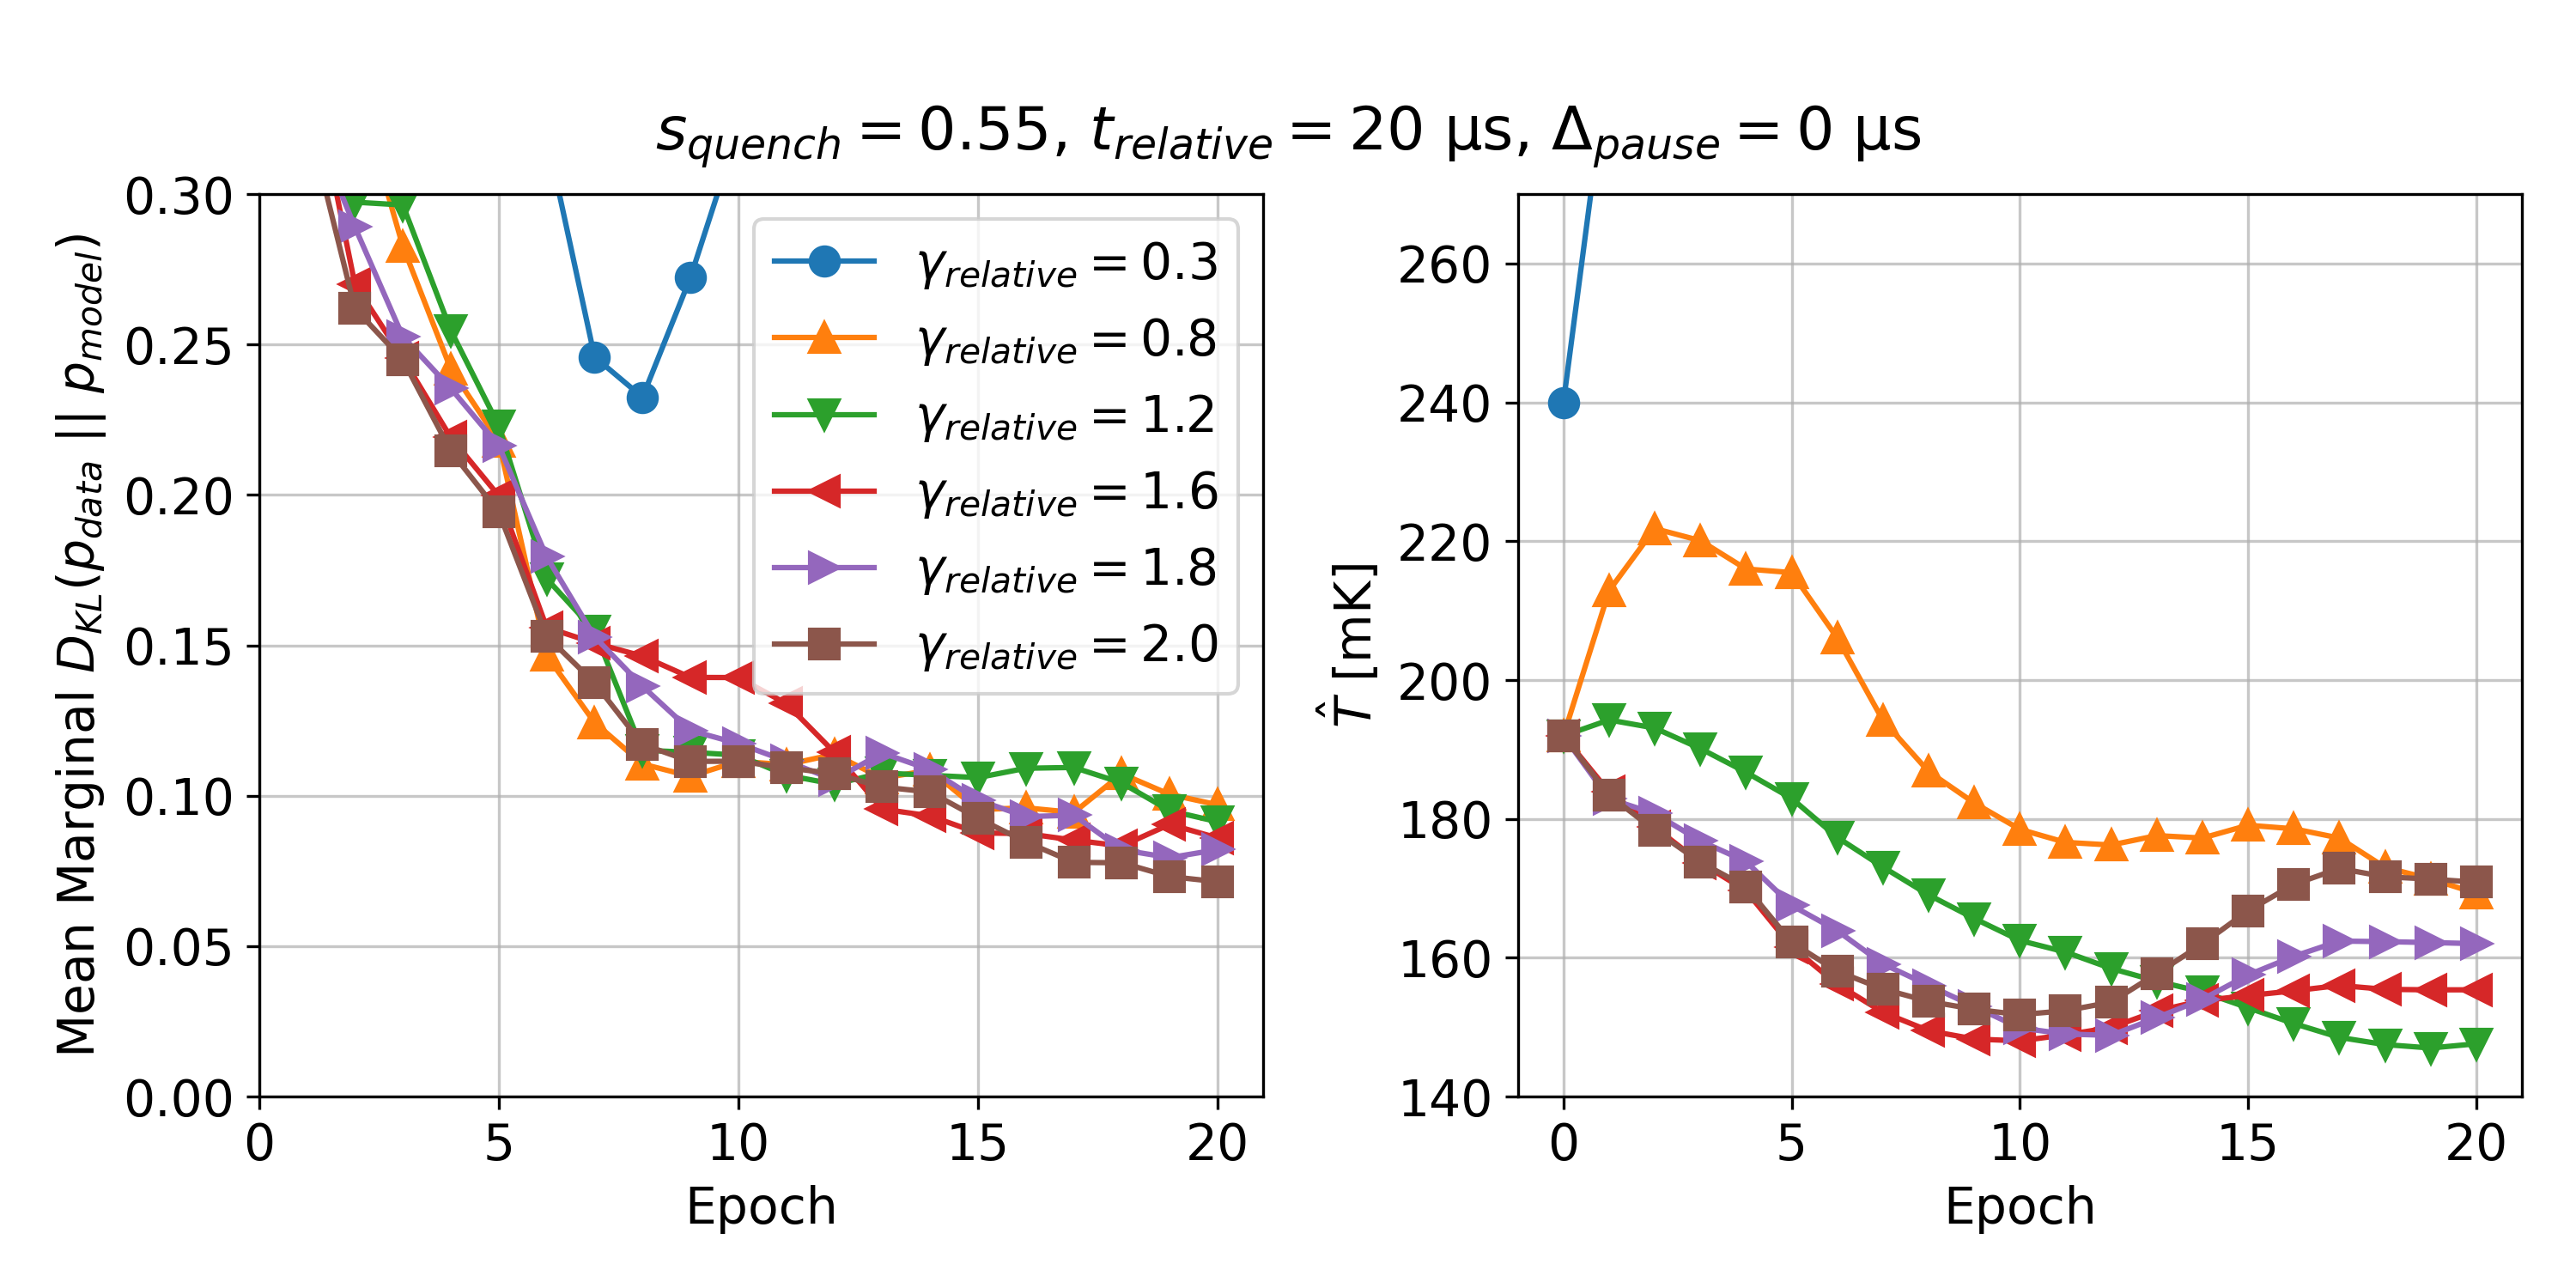
\includegraphics[width=1\linewidth]{qbm/log_returns/rcs_comparison.png}
    \end{center}
    \caption{
        Training results of the relative chain strength \( \rcs \) scan for embedding 1.
        On the left are the mean marginal \( \DKL{\pdata}{\pmodel} \) values, i.e., the average of the KL divergences of the individual currency pairs.
        On the right are the learned estimates of the effective temperature.
        Data plotted on a 5 epoch simple moving average basis to reduce visual noise.
    }
    \label{fig:qbm_log_returns_rcs_comparison}
\end{figure}

\subsubsection{Choosing an Anneal Schedule}
We keep \( \trelative = 20 \ \si{\micro\second} \) and \( \Deltapause = 0 \ \si{\micro\second} \) as in the 12-qubit problem, but check to see if a different value of \( \squench \) improves performance.
We try values of \( \squench = 0.5, 0.55, 0.6 \), plotted in~\cref{fig:qbm_log_returns_s_quench_comparison}, and find that \( \squench = 0.55 \) leads to the best KL divergence curve, and thus choose that value going forward.

\begin{figure}[!htb]
    \begin{center}
        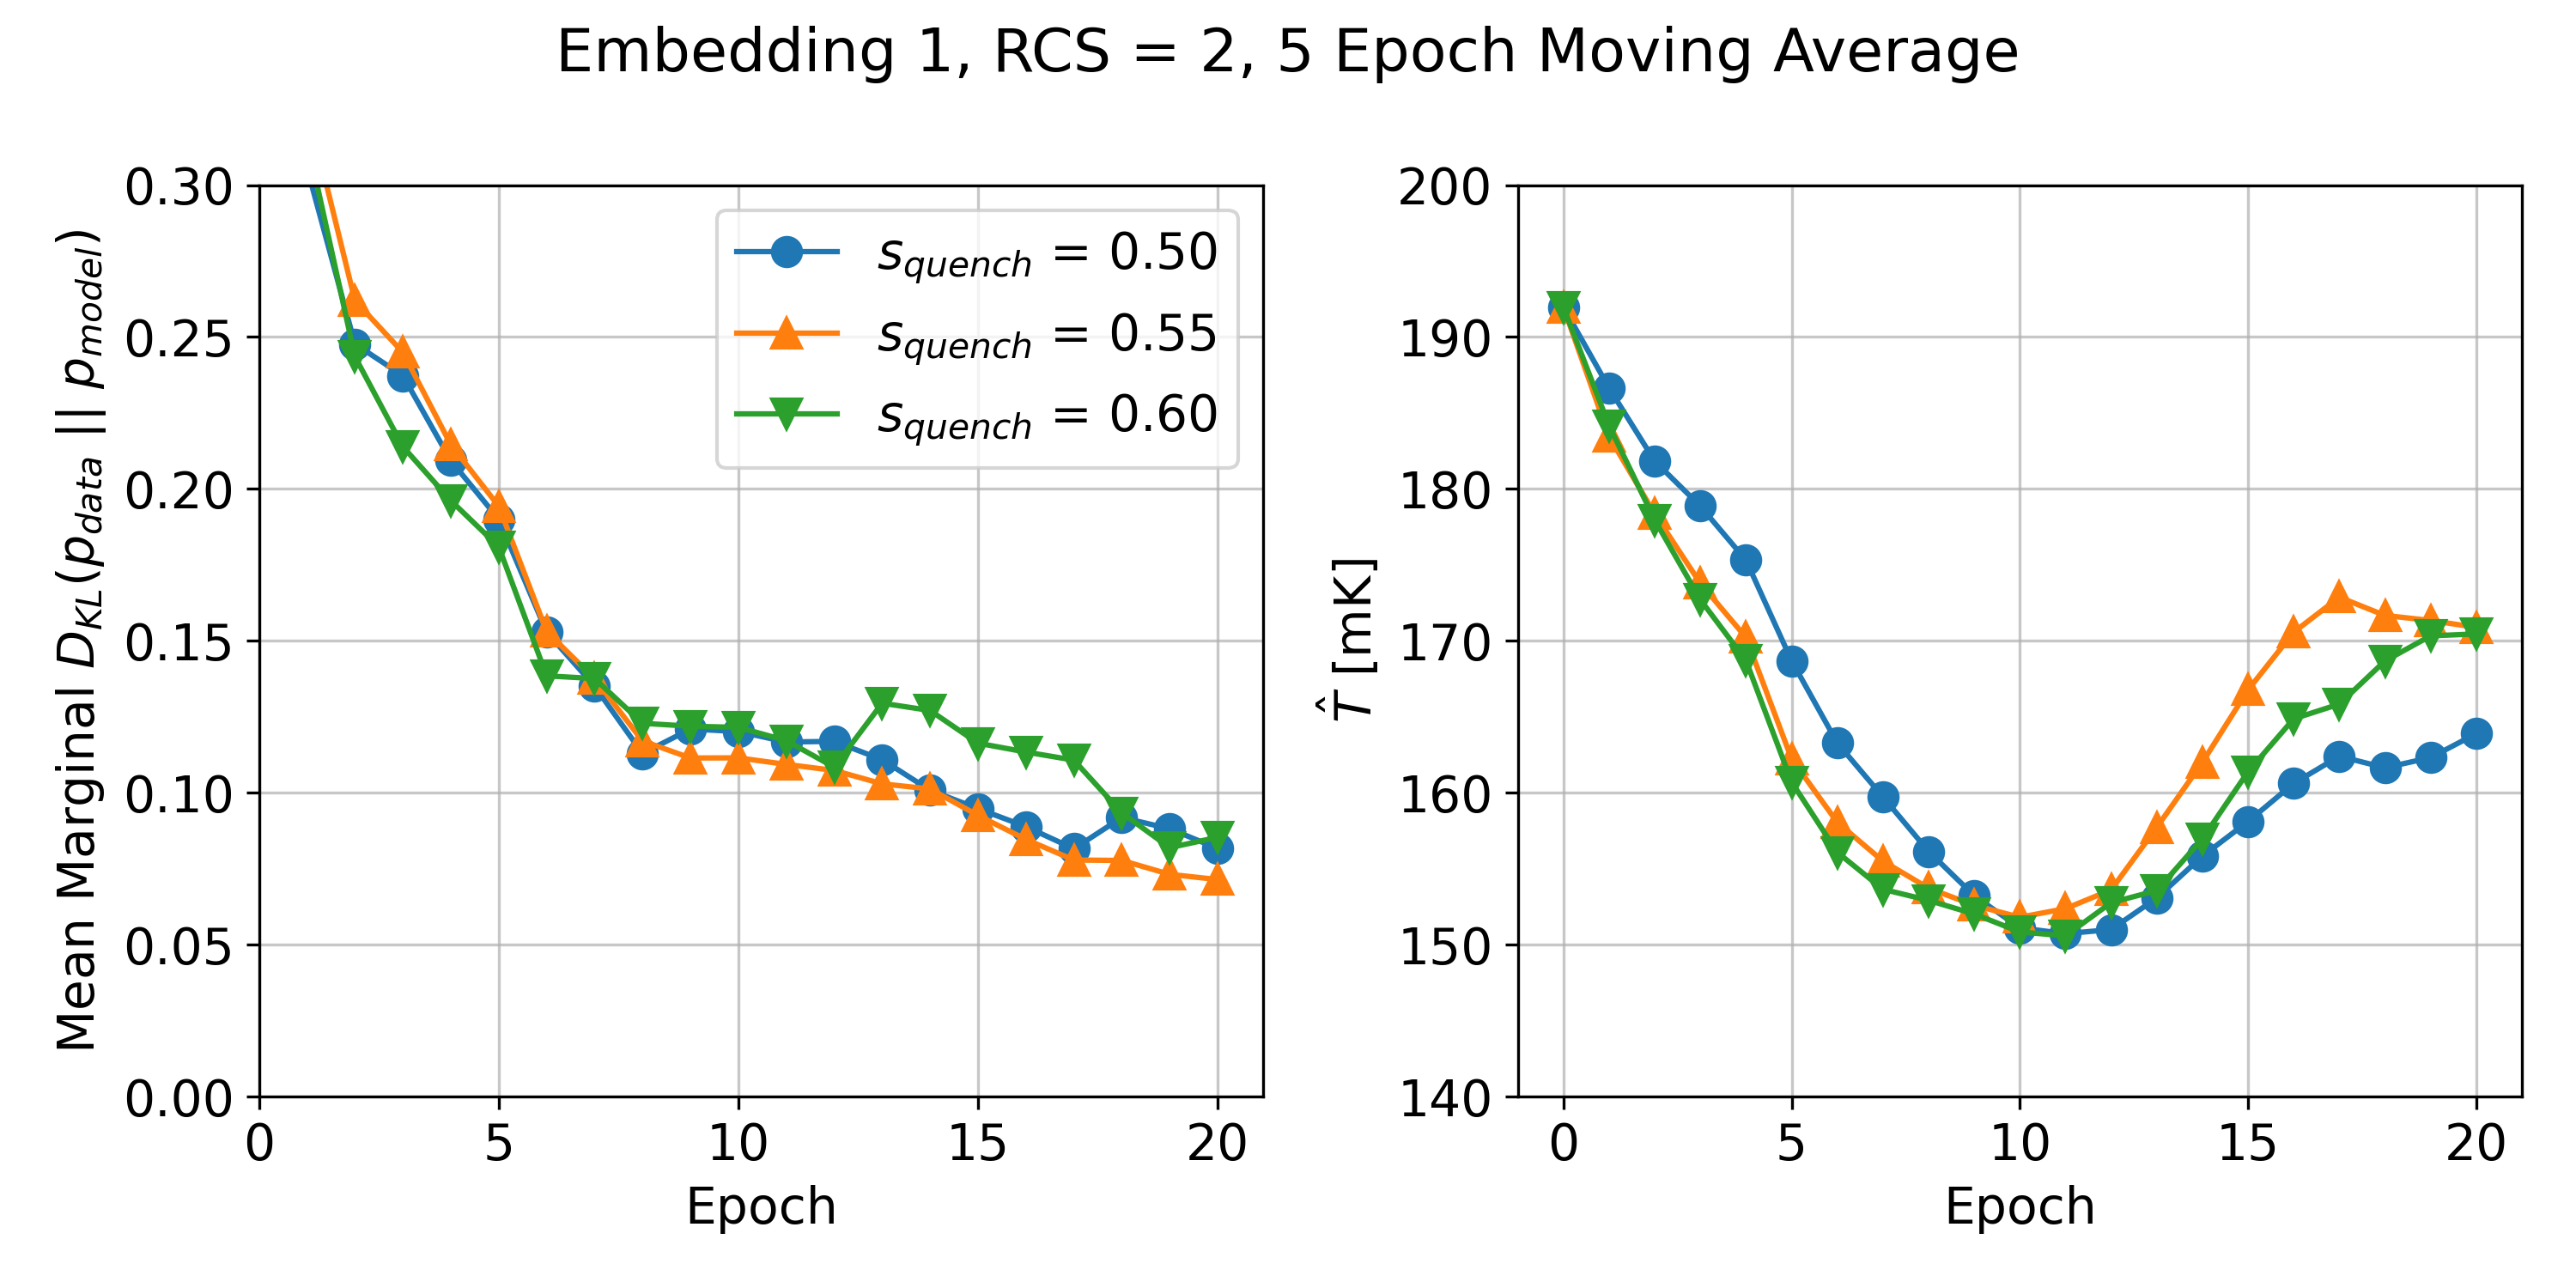
\includegraphics[width=1\linewidth]{qbm/log_returns/s_quench_comparison.png}
    \end{center}
    \caption{
        Training results of the \( \squench \) scan for embedding 1.
        On the left are the mean marginal \( \DKL{\pdata}{\pmodel} \) values, i.e., the average of the KL divergences of the individual currency pairs.
        On the right are the learned estimates of the effective temperature.
        Data plotted on a 5 epoch simple moving average basis to reduce visual noise.
    }
    \label{fig:qbm_log_returns_s_quench_comparison}
\end{figure}

\subsubsection{Choosing an Embedding}
The final annealer hyperparameter we seek to tune is the embedding.
We try 5 different heuristically generated embeddings each composed of around 400 physical qubits and maximum chain lengths of 7.
The comparison plotted in \cref{fig:qbm_log_returns_embedding_comparison} indicates to us that embedding 1 is likely a good choice to continue with.

\begin{figure}[!htb]
    \begin{center}
        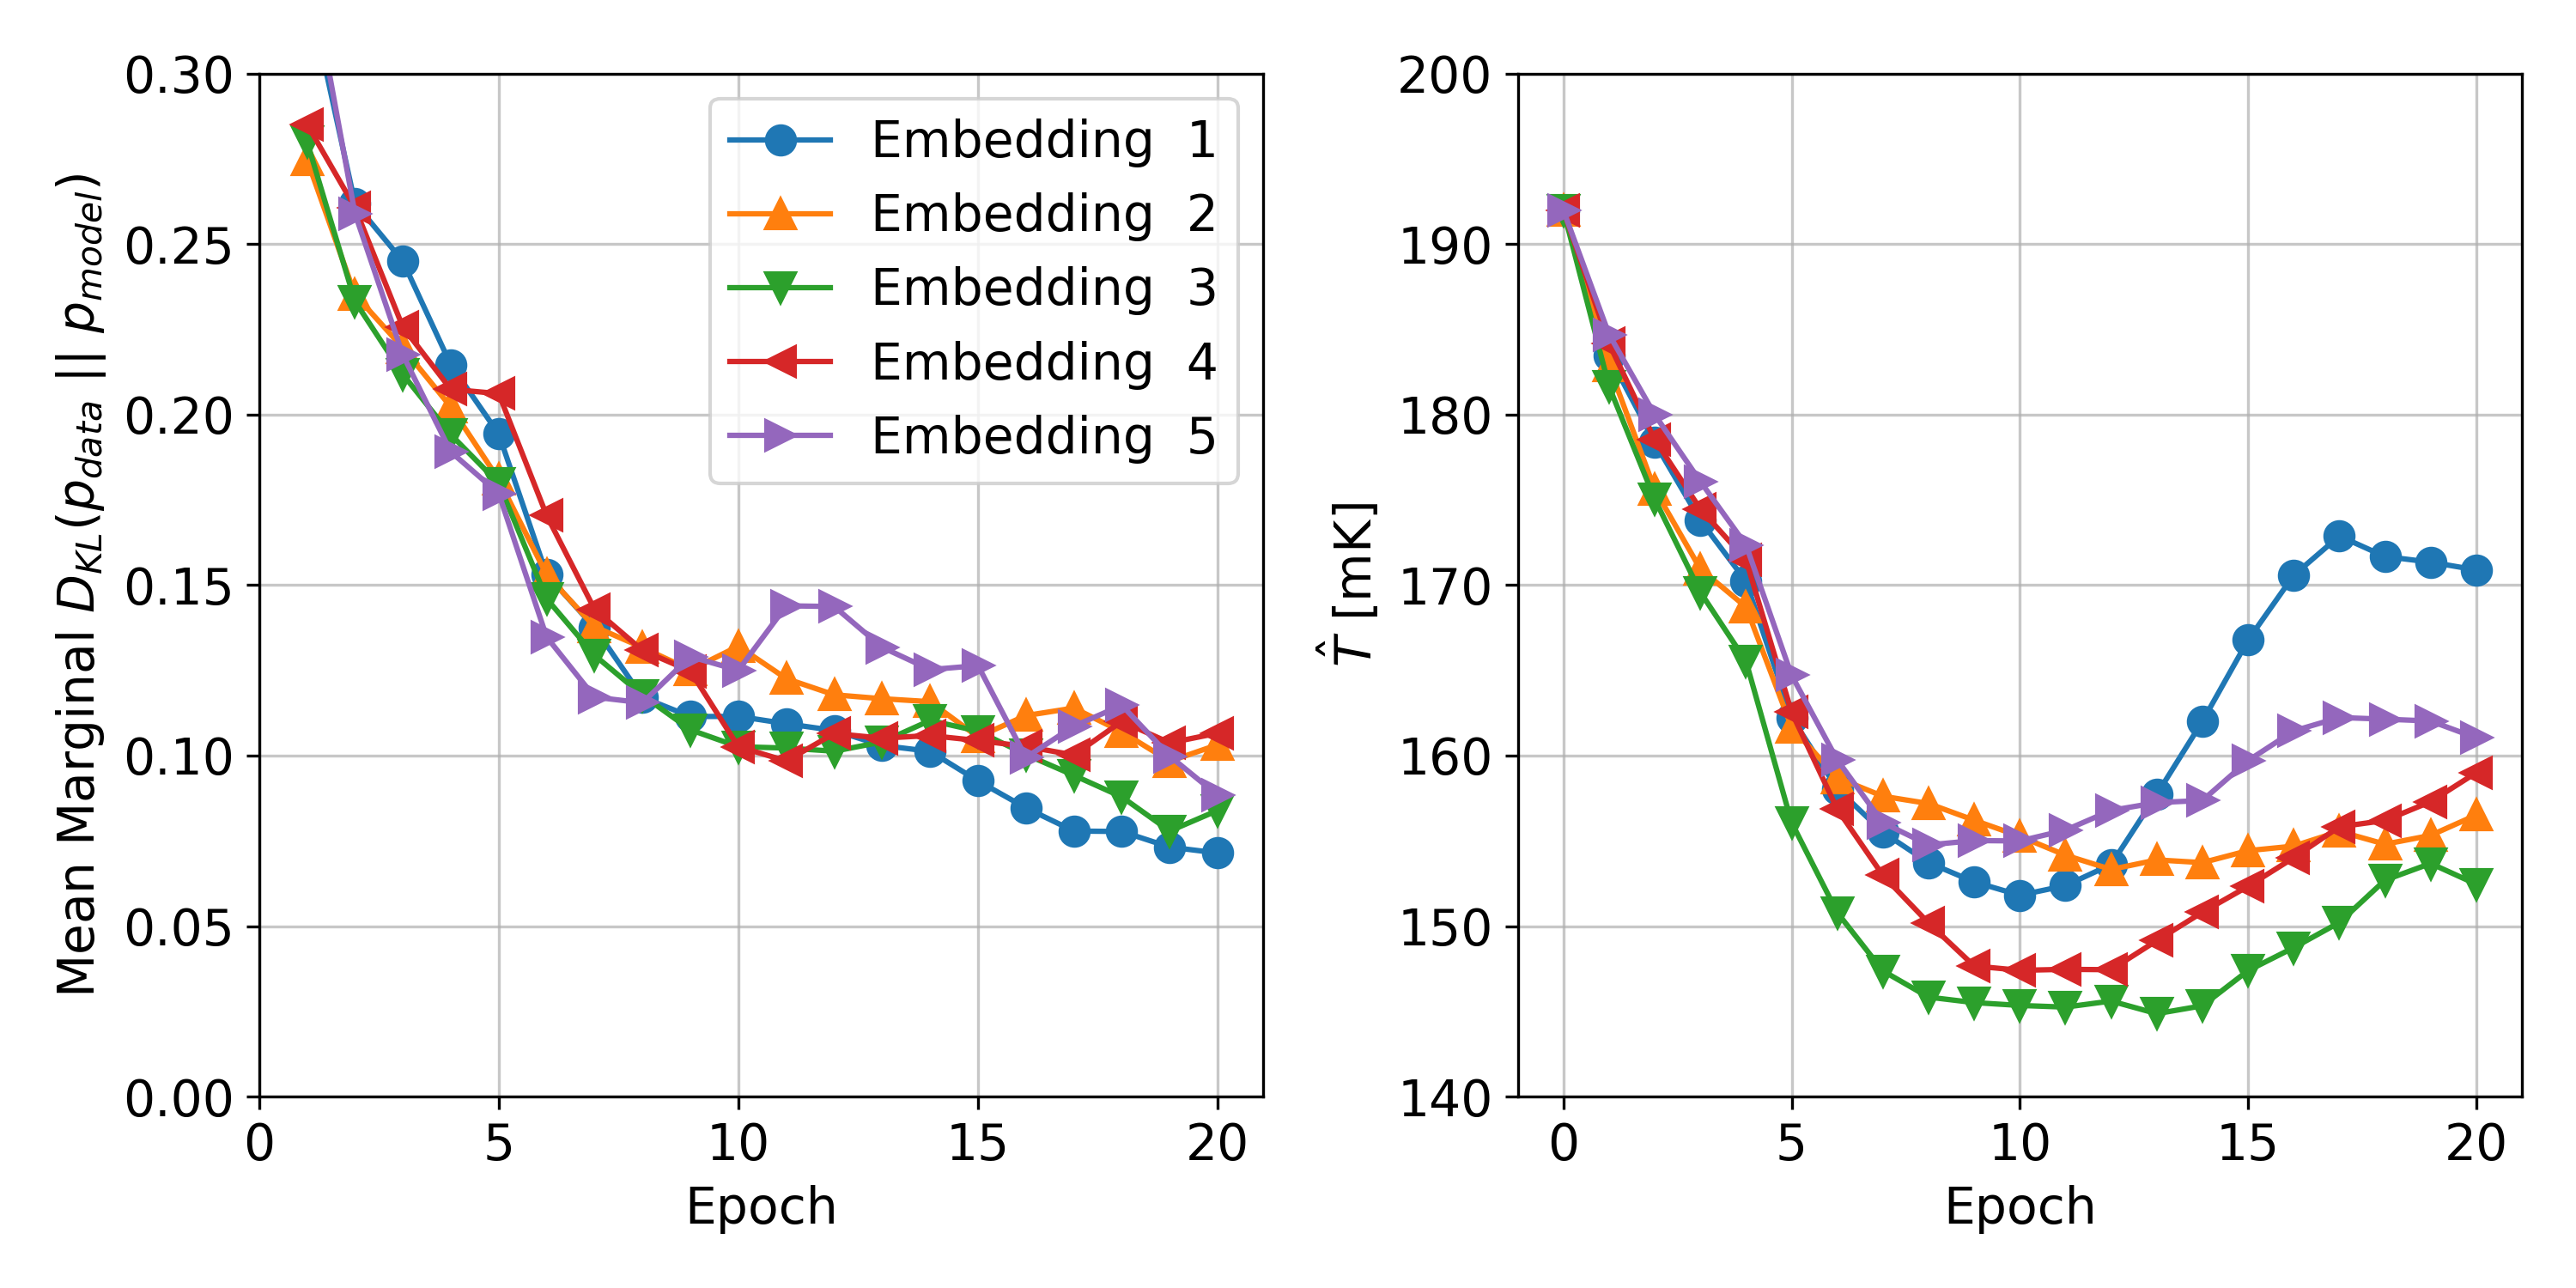
\includegraphics[width=1\linewidth]{qbm/log_returns/embedding_comparison.png}
    \end{center}
    \caption{
        Training results comparing 5 different embeddings.
        On the left are the mean marginal \( \DKL{\pdata}{\pmodel} \) values, i.e., the average of the KL divergences of the individual currency pairs.
        On the right are the learned estimates of the effective temperature.
        Data plotted on a 5 epoch simple moving average basis to reduce visual noise.
    }
    \label{fig:qbm_log_returns_embedding_comparison}
\end{figure}

\subsection{Results}\label{sec:qbm_log_returns_results}
With annealer hyperparameters of \( \rcs = 2 \), \( \squench = 0.55 \), and embedding 1, we move to training a full model over 100 epochs.
The training curves are depicted in~\cref{fig:qbm_log_returns_full_run}, where we observe the KL divergence decrease until around epoch 40 where it then oscillates for the remainder of the training process.
Unfortunately, the training results show that the BQRBM model significantly underperforms the classical model.

\begin{figure}[!htb]
    \begin{center}
        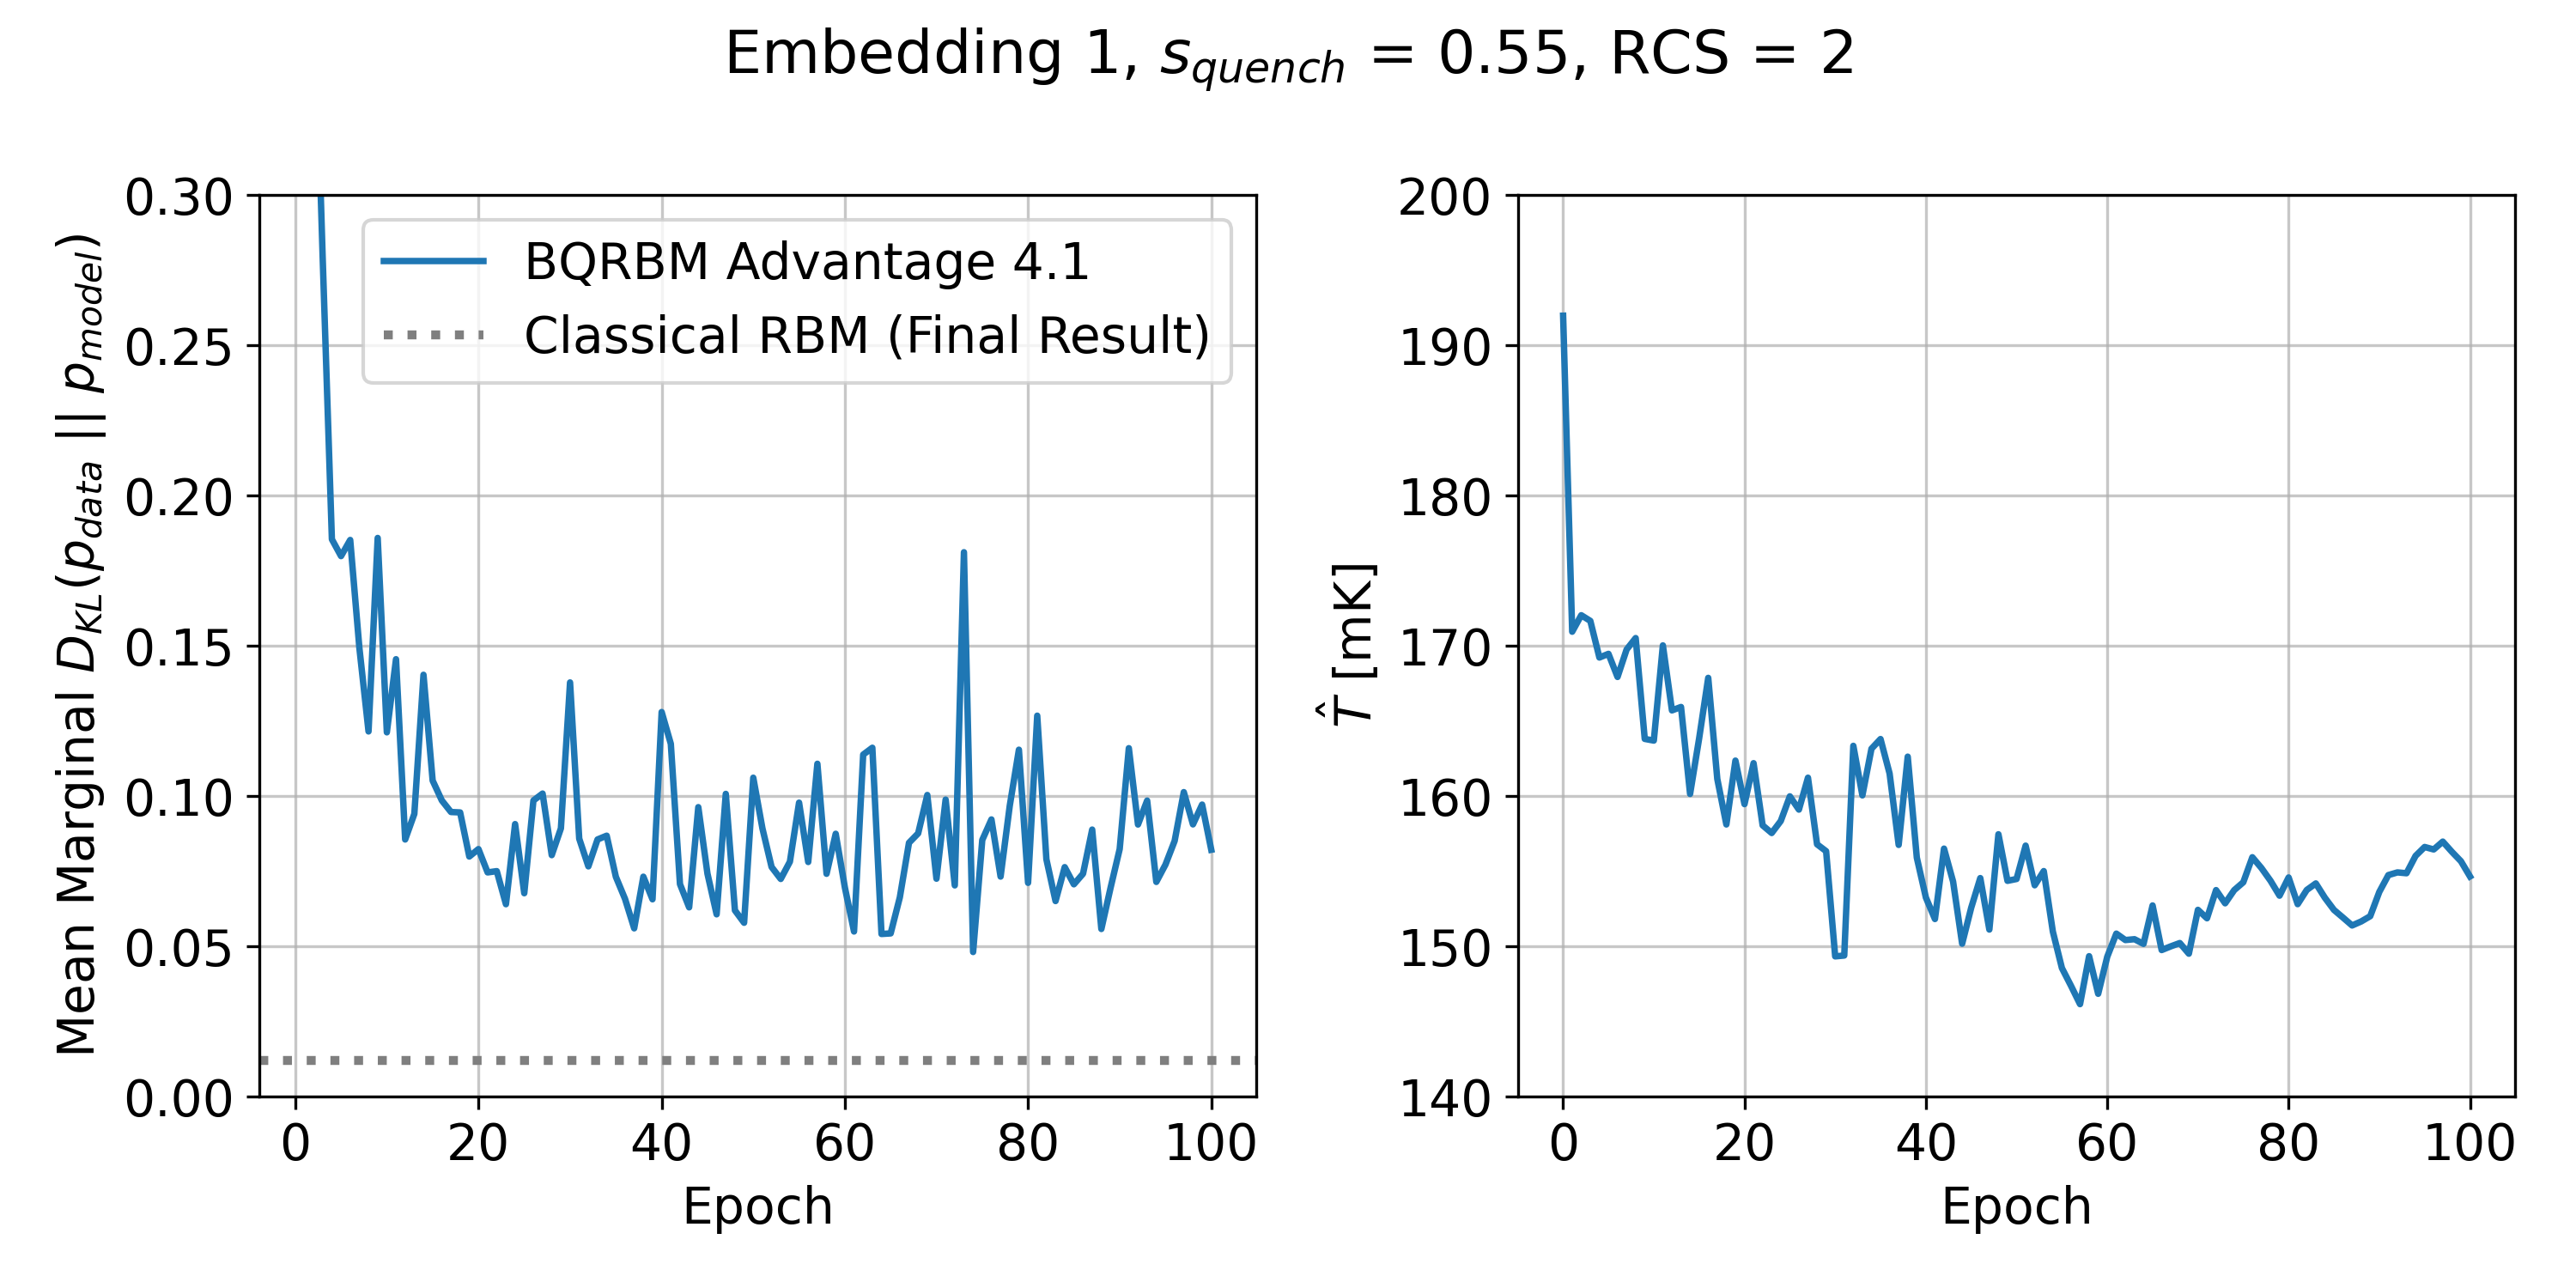
\includegraphics[width=1\linewidth]{qbm/log_returns/full_run.png}
    \end{center}
    \caption{
        Training results of the BQRBM compared with the final results of the classical RBM.
        On the left is the mean marginal \( \DKL{\pdata}{\pmodel} \) value, i.e., the average of the KL divergences of the individual currency pairs.
        On the right is the learned estimate of the effective temperature.
    }
    \label{fig:qbm_log_returns_full_run}
\end{figure}

Poor model performance is further confirmed by the KL divergences in~\cref{tbl:qbm_KL_divergences}.
We see the KL divergences of the BQRBM are about eight times higher than those of the classical RBM.
\begin{table}[!htb]
    \centering
    \begin{adjustbox}{max width=\textwidth}
        \input{../tables/qbm/kl_divergences.tbl}
    \end{adjustbox}
    \caption{
        KL divergences of the BQRBM model vs.~the classical RBM.
        The values are shown in the format mean \(\pm\) one standard deviation from an ensemble of 100 sample sets consisting of \( 10^4 \) samples each.
}
    \label{tbl:qbm_KL_divergences}
\end{table}

The Q-Q plots in~\cref{fig:qbm_log_returns_qq} point out that the BQRBM model struggles the most with the USDJPY and USDCAD marginals.
\begin{figure}[!htb]
    \begin{center}
        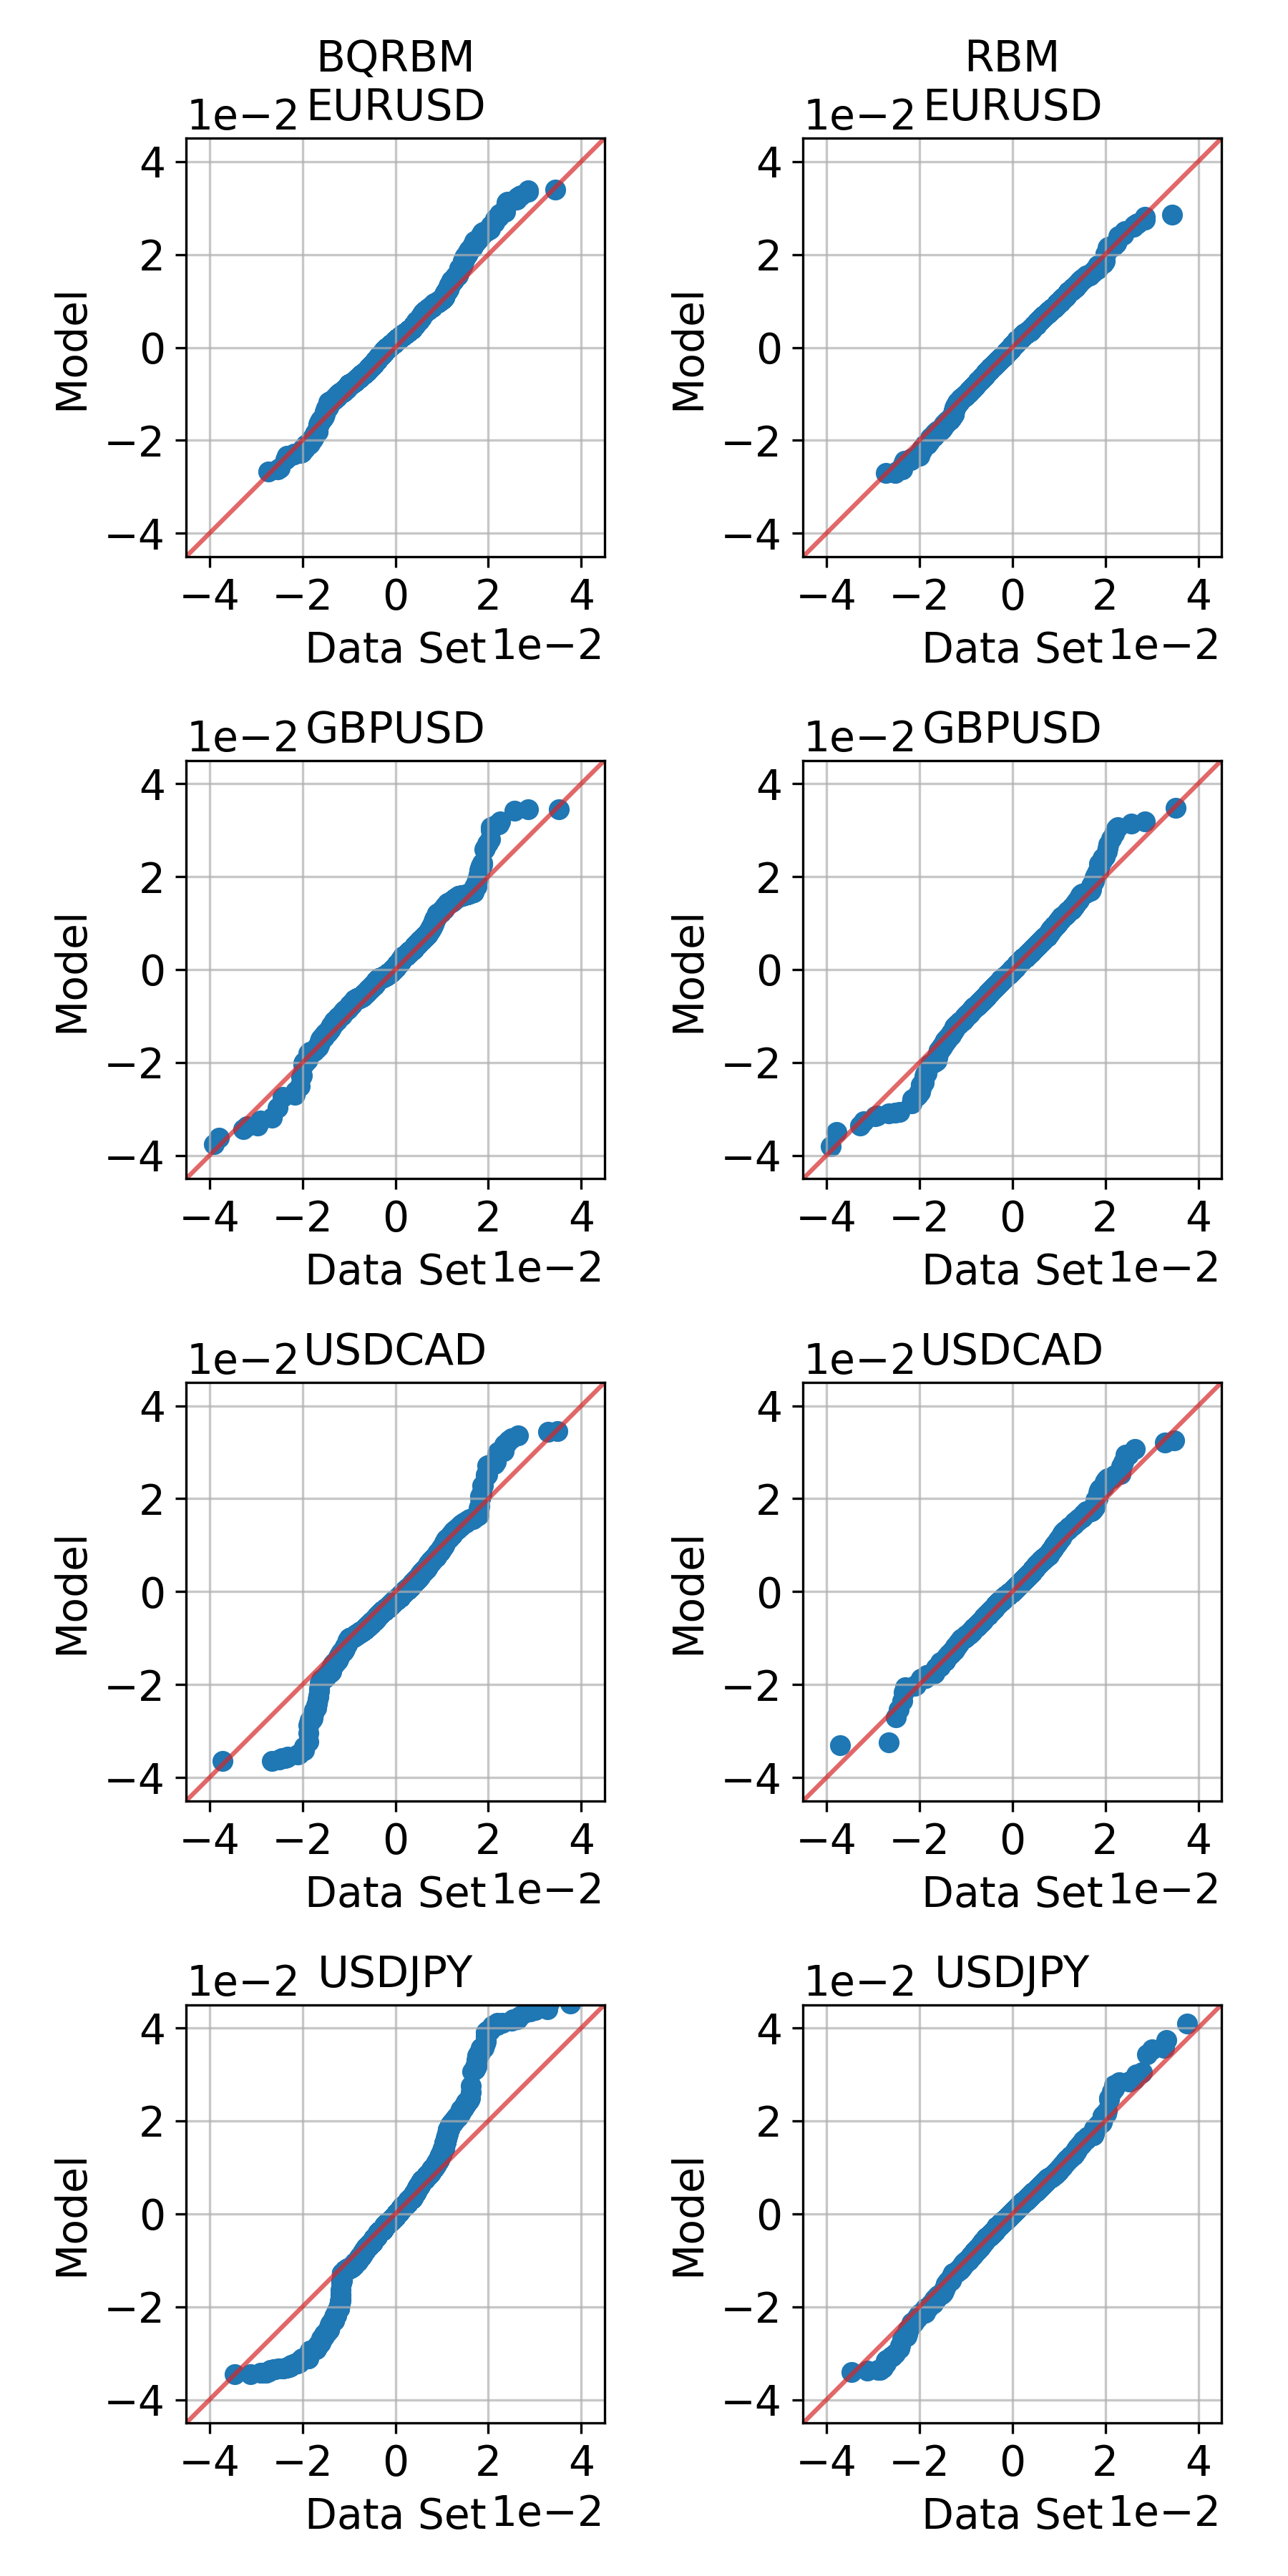
\includegraphics[width=0.7\linewidth]{qbm/log_returns/qq.png}
    \end{center}
    \caption{Log return Q-Q plots of the BQRBM and classical RBM models for each currency pair. Note that these plots only use the same number of samples as the size of the training data set (5165), and thus are not entirely representative of the models' performances.}
    \label{fig:qbm_log_returns_qq}
\end{figure}

\cref{tbl:qbm_correlation_coefficients} show that the BQRBM is able to reproduce the structure of the correlation coefficients, albeit to a lesser extent than the classical RBM.
\begin{table}[!htb]
    \centering
    \begin{adjustbox}{max width=\textwidth}
        \input{../tables/qbm/correlation_coefficients.tbl}
    \end{adjustbox}
    \caption{Correlation coefficients of the data set vs.~samples generated by the BQRBM and classical RBM models. The BQRBM and RBM values are shown in the format mean \(\pm\) one standard deviation from an ensemble of 100 sample sets consisting of \( 10^4 \) samples each.}
    \label{tbl:qbm_correlation_coefficients}
\end{table}

Interestingly, the BQRBM is able to reproduce the volatilities for the most part except for the USDJPY, as seen in~\cref{tbl:qbm_volatilities}.
\begin{table}[!htb]
    \centering
    \begin{adjustbox}{max width=\textwidth}
        \input{../tables/qbm/volatilities.tbl}
    \end{adjustbox}
    \caption{
        Historical volatilities of the data set vs.~samples generated by the BQRBM and classical RBM models.
        The BQRBM and RBM values are shown in the format mean \(\pm\) one standard deviation from an ensemble of 100 sample sets consisting of \( 10^4 \) samples each.
    }
    \label{tbl:qbm_volatilities}
\end{table}

\cref{tbl:qbm_tails} shows the quantum model struggles more on the tails, particularly with the USDJPY, as well as EURUSD.
This is further confirmed by the tail concentration functions in~\cref{fig:qbm_log_returns_tail_concentrations}.
\begin{table}[!htb]
    \centering
    \begin{adjustbox}{max width=\textwidth}
        \input{../tables/qbm/tails.tbl}
    \end{adjustbox}
    \caption{
        Lower and upper tails, i.e., 1st and 99th percentiles, of the data set vs.~samples generated by the BQRBM and classical RBM models.
        The BQRBM and RBM values are shown in the format mean \(\pm\) one standard deviation from an ensemble of 100 sample sets consisting of \( 10^4 \) samples each.
    }
    \label{tbl:qbm_tails}
\end{table}

\begin{figure}[!htb]
    \begin{center}
        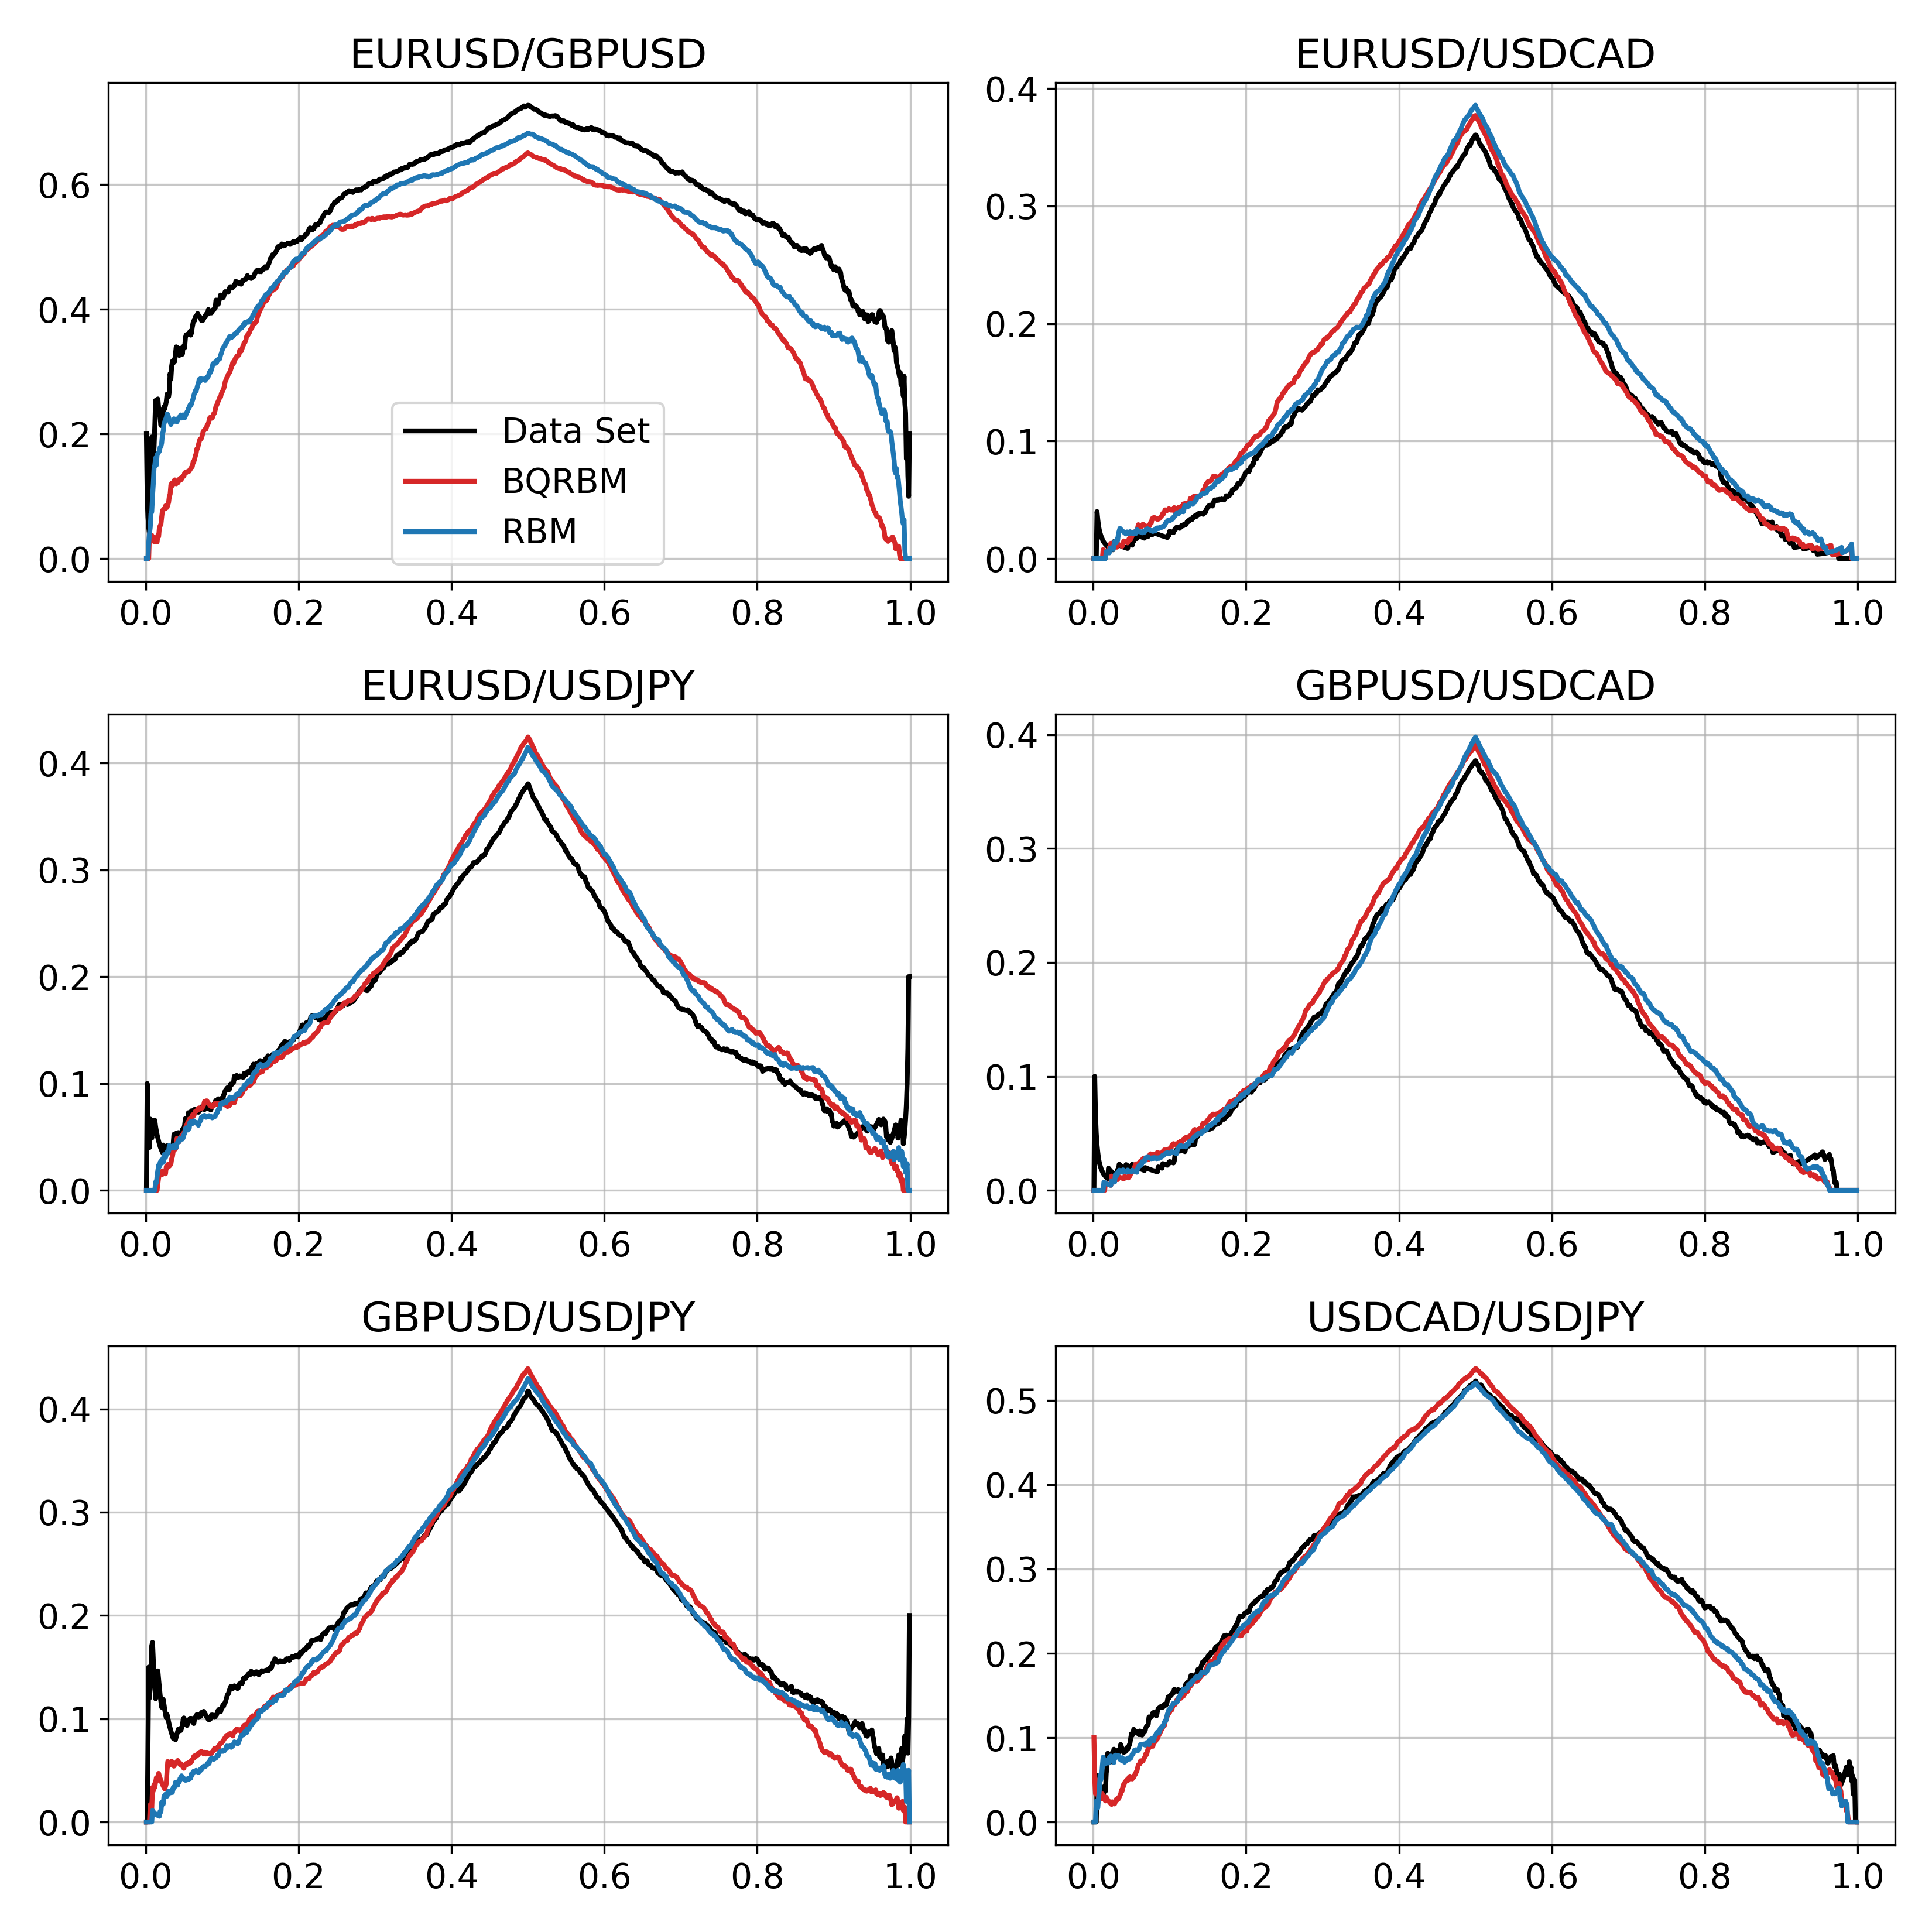
\includegraphics[width=1\linewidth]{qbm/log_returns/tail_concentrations.png}
    \end{center}
    \caption{Tail concentration functions of the data set vs.~samples generated by the BQRBM and classical RBM models.}
    \label{fig:qbm_log_returns_tail_concentrations}
\end{figure}

\subsection{Summary}
Overall, the BQRBM model trained using the Advantage 4.1 produces lackluster results when compared with the classical RBM, and does not motivate training additional models on the transformed and volatility indicator enhanced data sets.
This could possibly be due to hyperparameters, as our grid search of the space was not the most optimal due to training time requirements, but it is not immediately clear if there is a better way to do this.
This could also be due to the fact that the model is so large that it uses a significant portion of the QPU and requires chains with lengths of up to 7, resulting in added complexity.

In conclusion, it does not appear that the Advantage 4.1-trained BQRBM can produce results good enough to replace the classical RBM.
It will be interesting to see how much this improves with future generations of annealers, although it will likely take serious advances in the technology to outperform the classical RBM.

\clearpage
\section{Challenges of Using a D-Wave Annealer to Train QBMs}\label{sec:challenges}
Using a D-Wave quantum annealer to train quantum Boltzmann machines is a difficult task, and there are many challenges which need to be overcome in order to do so.
In this section we touch on some of these difficulties and discuss some possible methods to mitigate them.
Around the time this thesis was started, Pochart et al. released a paper~\cite{pochart_2021} in which they discuss challenges associated with using a D-Wave annealer to sample Boltzmann random variables.

\subsection{Choosing an Embedding}
Mapping the logical qubits to physical qubits is nontrivial.
D-Wave provides a heuristic method to find embeddings, but in practice it cannot be guaranteed that the returned embedding is optimal.
As we saw first hand, different embeddings can produce different results.
Therefore, it is recommended to generate multiple embeddings and compare them against each other, and choose the one that performs the best.
Additionally, it is worth noting that an optimal embedding on one QPU might not be optimal on another of the same generation.

\subsubsection{Chain Strength}
Depending on how large the problem is, one will likely need to use an embedding that is not direct, i.e., one that requires chains of physical qubits to represent single logical qubits due to limited connectivity.
This brings about an additional hyperparameter that needs to be tuned.
Rather than setting the chain strength directly though, it is recommended to use the relative chain strength as mentioned in~\cref{sec:qbm_rcs}.
It is best to do a comparison in the beginning to get an idea of what a good relative chain strength might be, as it is problem dependent.

\subsection{Sampling the Proper Distribution}
The most important thing when using a quantum annealer to train a Boltzmann machine is making sure the annealer is sampling from the proper distribution.
In the case of the quantum Boltzmann machine we need samples generated according to \( \rho = \frac{1}{Z} e^{-\beta H(s^*)} \).
For smaller problems it is easy to compare results obtained from the annealer with exact computed distributions (as we did for the 12-qubit problem), but it is not as simple for larger problems.
For larger problems there is the possibility to use advanced methods, such as they did in~\cite{marshall_2019} with the use of an entropic sampling technique~\cite{barash_2019} based on population annealing to estimate degeneracies, and in turn use those to compute classical Boltzmann distributions to compare with, but that might not always be practical.
Alternatively, one can try a hyperparameter grid search as we did in~\cref{sec:qbm_hyperparameters}

\subsubsection{Effective Temperature}
One of the most important hyperparameters is that of the effective inverse temperature \( \beta \).
In practice, we divide our weights and biases by a factor of \( -\betahat B(s^*) \) (as per~\cref{eq:qbm_scaling}) in order to cancel out the effective temperature so that we can sample the problem we wish to, thus it is crucial for proper parameter scaling.
For the case of \( s^* = 1 \) we have the ability to treat the effective temperature as a learnable parameter (as in~\cref{sec:learning_beta}), for which we use \( \betahat \) as an estimator of.
This is not so straightforward for \( s^* < 1 \) though, because of the initial Hamiltonian and the D-Wave's inability to measure the qubits in the \( x \)-direction.

\subsubsection{Anneal Schedules}
The ability to configure the anneal schedule as allowed by the D-Wave annealer means that there are a number of different ways one can tweak the annealing process such that the results returned minimize the KL divergence between the theoretical distribution one wishes to approximate and the samples returned by the annealer.
In an ideal world, the way to get the desired distribution is to anneal slowly at first, then quench the system at the point \( s^* \) and measure the qubits~\cite{amin_2018}.
Unfortunately, the research conducted in this thesis seems to indicate that the current generation of D-Wave annealers cannot quench fast enough to prevent any nontrivial dynamics occurring after \( s^* \), and all sample sets we collected are more similar to classical Boltzmann distributions than quantum ones.
With that said, the annealer can still be used to assist in the training of a classical Boltzmann machine.

\subsection{QPU Limitations and Imperfections}
The properties of the QPU itself must also be taken into account.
There is no doubt that D-Wave is a top-notch manufacturer of quantum annealers, but even with all of their expertise the QPUs are still subject to imperfections and errors.
It is possible for some areas of the chip to perform better than others, or for some of the qubits to have readout biases (although biases can be mitigated by using gauge transforms as detailed in~\cref{sec:gauge}).

\subsubsection{Maximum Sample Set Size}
One of the main limitations of the D-Wave annealer for this purpose is that of the maximum sample set size.
When sampling the D-Wave one can only generate sample sets with a maximum size of \( 10^4 \) samples, which is adequate for the intended purpose of optimization, but can fall short when one wants to use it as a sampler for a QBM.
It is natural to think that one could just combine the results from multiple sample sets, but this is not necessarily the case.
Due to the spin-bath polarization effect (see error sources below), one cannot combine sample sets because of the possibility of previous samples affecting future ones~\cite{pochart_2021}.

\subsubsection{Time Requirements}
Another issue is the time requirements.
Most models detailed here require little QPU access time, around 5-10 minutes, but this can add up and get expensive if one is doing a hyperparameter grid search.
Additionally, there is the total training time, which as we saw can be quite substantial due the latency to the cloud platform combined with the load queue of the solver.
To illustrate this point, training the simulation-based 12-qubit model takes roughly 2 seconds per epoch (the majority of which is spent computing the density matrix), whereas the Advantage 4.1-based model takes 2-5 minutes per epoch.

\subsubsection{Error Sources}
There are a number of sources from which errors can arise on a D-Wave quantum annealer.
D-Wave does an excellent job at detailing these errors in their documentation~\cite{dwave_ice_errors,dwave_other_errors}, so we will only briefly touch on them here with high-level information obtained from the aforementioned references.
\begin{itemize}
    \item \textbf{Integrated Control Errors (ICE)} are errors due to the accuracy at which the \( h_i \) and \( J_{ij} \) values can be implemented.
        In mathematical terms this is because the problem the QPU solves is closer to
        \begin{align}
            H_{\text{Ising}}^\delta = \sum_{i=1}^{n} (h_i + \delta_{h_i}) \sigma_i^z + \sum_{i=1}^{n}\sum_{j=i+1}^n (J_{ij} + \delta_{J_{ij}}) \sigma_i^z \sigma_j^z,
        \end{align}
        for some small \( \delta_{h_i} \) and \( \delta_{J_{ij}} \).
    \item \textbf{Temperature} errors arise due to fluctuations in the physical temperature of the device, which can change depending on how frequently the QPU is programmed.
    \item \textbf{High-Energy Photon Flux} errors can occur in the presence of photons with energies higher than that expected at the effective temperature dependent equilibrium, which can lead to higher energy solutions. These photons originate from cryogenic filtering at higher temperature phases.
    \item \textbf{Readout Fidelity} errors can occur when the bit string returned by the annealer differs from that arrived at by the QPU by one or more bit flips.
        For reference, D-Wave annealers have a readout fidelity of >99\%.
    \item \textbf{Programming Errors} can occur when the problem implemented by the QPU suffers from programming issues resulting in the implemented problem's low-energy subspace not having an overlap with that of the desired problem.
    \item \textbf{Spin-Bath Polarization Effect} errors can arise when the current flowing through the qubits during the annealing process cause the spins to obtain a polarization which can bias the measurements.
\end{itemize}
